\chapter{Verification and validation}

\section{Evaluation metrics for image compression}\label{sec:eval_metrics}
For evaluating the performance of training and validating image compression models, appropriate metrics are needed to quantify the quality of compressed images.
Some of the most common metrics used in HSI compression are Peak Signal-to-Noise Ratio (PSNR), Structural Similarity Index Measure (SSIM), Mean Squared Error (MSE), and Spectral Angle (SA)\cite{mohammadi2025evaluationobjectiveimagequality, SA}.
These metrics help to quantify the differences between the original and reconstructed images, providing insights into the effectiveness of models used for compression.
Two metrics are particularly well suited for examining HSI compression performance, SA and SSIM.
PSNR and MSE are more general metrics often used in image processing tasks.
MSE measures the average squared difference between the original and reconstructed pixel values, where PSNR is MSE logarithmic scale representation expressed in decibels (dB). \cite{mohammadi2025evaluationobjectiveimagequality}
Unlike PSNR and the MSE, SSIM is a metric designed to align more closely with visual perception.
SSIM evaluates the similarity between two images based on their structural information, luminance, and contrast. \cite{mohammadi2025evaluationobjectiveimagequality}
SA measures the spectral similarity between the original and reconstructed image by calculating the angle between their spectral vectors. \cite{SA}

\subsection{Structural Similarity Index Measure}
The Structural Similarity Index Measure (SSIM) is a metric that quantifies many image quality aspects.
It combines data about the differences in luminance, contrast, and structure between two images into a single value.
The formula for calculating SSIM between two images \( x \) and \( y \) is given by equation \ref{fig:ssim_equation}:
\begin{align}
    \text{SSIM}(x, y) = \frac{(2\mu_x \mu_y + C_1)(2\sigma_{xy} + C_2)}{(\mu_x^2 + \mu_y^2 + C_1)(\sigma_x^2 + \sigma_y^2 + C_2)}
    \label{fig:ssim_equation}
\end{align}
where \( \mu_x \) and \( \mu_y \) are the average pixel values of images \( x \) and \( y \), \( \sigma_x^2 \) and \( \sigma_y^2 \) are the variances, \( \sigma_{xy} \) is the covariance between the two images, and \( C_1 \) and \( C_2 \) are constants to ensure no division by zero takes place.
The SSIM value theoretically ranges from -1 to 1, where a value of 1 indicates perfect similarity between the two images, while values close to 0 indicate low similarity and negative values indicate very opposite similarity.
In practice, for image compression tasks, SSIM values are typically between 0 and 1, with higher values indicating better reconstruction quality.
\subsection{Spectral Angle}
The formula for calculating the SA between two spectral vectors \( \mathbf{a} \) and \( \mathbf{b} \) is given by equation \ref{fig:sa_equation}:
\begin{align}
    \text{SA}(\mathbf{a}, \mathbf{b}) = \arccos\left(\frac{\mathbf{a} \cdot \mathbf{b}}{\|\mathbf{a}\|\|\mathbf{b}\|}\right)
    \label{fig:sa_equation}
\end{align}
where \( \mathbf{a} \cdot \mathbf{b} \) is the dot product of the vectors, and \( \|\mathbf{a}\| \) and \( \|\mathbf{b}\| \) are the magnitudes of the vectors.
SA is typically measured in degrees, with smaller angles indicating greater similarity between the spectral signatures.
\subsection{Mean Squared Error}
Mean Squared Error (MSE) is a common metric often used in machine learning.
It measures the average square of the difference of each point.
In the case of images, it measures the average squared difference between the original and reconstructed pixel values.
The formula for calculating MSE between two images \( x \) and \( y \) is shown in equation \ref{fig:mse_equation}:
\begin{align}
    \text{MSE}(x, y) = \frac{1}{N} \sum_{i=1}^{N} (x_i - y_i)^2
    \label{fig:mse_equation}
\end{align}
where \( N \) is the total number of pixels in the images, and \( x_i \) and \( y_i \) are the pixel values at position \( i \).
The MSE value is non-negative, with lower values indicating better reconstruction quality.
\subsection{Peak Signal-to-Noise Ratio}
Peak Signal-to-Noise Ratio (PSNR) is a metric used to measure the quality of reconstructed images compared to the original images.
It is expressed in decibels (dB) which are logarithmic units.
This, in turn, means that small changes in PSNR can represent significant differences in image quality.
The formula for calculating PSNR between two images \( x \) and \( y \) is given by equation \ref{fig:psnr_equation}:
\begin{align}
    \text{PSNR}(x, y) = 10 \cdot \log_{10} \left( \frac{MAX_I^2}{\text{MSE}(x, y)} \right)
    \label{fig:psnr_equation}
\end{align}
where \( MAX_I \) is the maximum possible pixel value of the image.
The PSNR value is better when it is higher, with values above 30 dB generally considered good enough for most image compression tasks, while values above 45 dB are considered excellent.
It is important to note that PSNR is a logarithmic measure, so a small increase in PSNR can correspond to a significant improvement in image quality.
\subsection{Bits per pixel per channel}
Another metric specific to HSIs is the bits per pixel per channel (bpppc), which represents the average number of bits used to encode each pixel in each spectral channel.
The formula for calculating bpppc is given by equation \ref{fig:bpppc_equation}:
\begin{align}
    \text{bpppc} = \frac{\text{Total Bits in Compressed Image}}{\text{Number of Pixels} \times \text{Number of Spectral Channels}}
    \label{fig:bpppc_equation}
\end{align}
The bpppc metric is particularly important for evaluating the efficiency of compression algorithms, as it directly relates to the amount of data required to represent the image.
Lower bpppc values indicate more efficient compression, while higher values indicate less efficient compression.

\subsection{Error histogram}
Besides numerical metrics, visualizing the distribution of reconstruction errors was employed to gain insights into the typical errors made by the compression models.
Visualizing the distribution of reconstruction errors can be achieved in the form of a histogram.
The histograms present the frequency of errors over some interval, which provides a way to identify patterns in the errors.
For instance, a histogram that is heavily skewed toward zero indicates that most reconstruction errors are small, suggesting that the model is performing well.
A histogram with a peak away from zero indicates that the model is frequently making larger errors, which may suggest areas for improvement.
The best error histogram would ideally show a high frequency of errors close to zero, indicating that the model is accurately reconstructing the images with minimal errors.

\subsection{Error map}
An additional method for visualizing reconstruction errors is through error maps.
Error maps are the result of calculating the difference between the original and reconstructed images on a pixel-by-pixel basis.
These maps provide a spatial representation of where the model is performing well and where it is struggling.
The error maps presented in this thesis use a color scale to represent the magnitude of the errors.
Pixels with negative errors are shown in shades of blue, while pixels with positive errors are shown in shades of red, and black represents zero error.
This color scheme allows for easy identification of areas where the model is overestimating or underestimating pixel values.

\section{Evaluation of semantic segmentation} \label{sec:segmentation_eval}
To evaluate the performance of the semantic segmentation model, several common metrics were used, including the confusion matrix, accuracy, positive predictive value (PPV), recall, F1-score, Intersection over Union (IoU), and Area under Curve (AUC).
These metrics provide a comprehensive assessment of the model's ability to correctly assign classes to each pixel in the image.
% ROZWINAC

\subsection{Confusion matrix}
A confusion matrix is a table that summarizes the performance of a classification model by comparing the predicted class labels with the true class labels.
Each row of the matrix corresponds to the true class (as labeled in the dataset), while each column corresponds to the predicted class (as output by the model).
The entries in the matrix represent the number of pixels that were classified into each combination of true and predicted classes.
The perfect model would produce a diagonal confusion matrix, where all pixels are correctly classified into their respective classes.\par
The confusion matrix provides a detailed view of the model's performance, allowing for the identification of specific classes that may be more challenging to classify correctly.
Another useful aspect of the confusion matrix is that it can be used to calculate other evaluation metrics such as accuracy, precision, recall, and F1-score.
This can be done by summing the appropriate entries in the matrix to obtain the necessary counts for each metric.
All of these summations fall into four categories: true positives (TP), true negatives (TN), false positives (FP), and false negatives (FN).
True positives are the number of pixels that were correctly classified as belonging to a particular class.
True negatives are the number of pixels that were correctly classified as not belonging to a particular class.
False positives are the number of pixels that were incorrectly classified as belonging to a particular class when they do not.
False negatives are the number of pixels that were incorrectly classified as not belonging to a particular class when they do.

\subsection{Accuracy}
Accuracy is a metric that measures the overall correctness of the model's predictions.
It is calculated as the ratio of correctly classified pixels to the total number of pixels in the image.
The formula for calculating accuracy is given by equation \ref{fig:accuracy_equation}:
\begin{align}
    \text{Accuracy} = \frac{TP + TN}{TP + TN + FP + FN}
    \label{fig:accuracy_equation}
\end{align}
The accuracy value ranges from 0 to 1, with higher values indicating better performance.

\subsection{Positive predictive value }
PPV is a metric that directly measures the proportion of positive identifications that were actually correct.
It is calculated as the ratio of true positives to the sum of true positives and false positives.
The formula for calculating PPV is given by equation \ref{fig:ppv_equation}:
\begin{align}
    \text{PPV} = \frac{TP}{TP + FP}
    \label{fig:ppv_equation}
\end{align}
The PPV value ranges from 0 to 1, with higher values indicating better performance.
\subsection{Recall}
Recall is a metric that measures the model's ability to correctly identify all relevant instances of a particular class.
It is calculated as the ratio of true positives to the sum of true positives and false negatives.
The formula for calculating recall is given by equation \ref{fig:recall_equation}:
\begin{align}
    \text{Recall} = \frac{TP}{TP + FN}
    \label{fig:recall_equation}
\end{align}
The recall value ranges from 0 to 1, with higher values indicating better performance.
\subsection{F1-score}
F1-score is a metric that combines PPV and recall into a single value.
It is the harmonic mean of PPV and recall, providing a balanced measure of the model's performance.
The formula for calculating F1-score is given by equation \ref{fig:f1_equation}:
\begin{align}
    \text{F1-score} = 2 \cdot \frac{\text{PPV} \cdot \text{Recall}}{\text{PPV} + \text{Recall}}
    \label{fig:f1_equation}
\end{align}
The F1-score value ranges from 0 to 1, with higher values indicating better performance.
\subsection{Intersection over Union}
IoU is a metric that measures the overlap between the predicted and true class labels.
It is calculated as the ratio of the intersection of the predicted and true class labels to the union of the predicted and true class labels.
The formula for calculating IoU is given by equation \ref{fig:iou_equation}:
\begin{align}
    \text{IoU} = \frac{TP}{TP + FP + FN}
    \label{fig:iou_equation}
\end{align}
The IoU value ranges from 0 to 1, with higher values indicating better performance.
\subsection{Area under Curve}
AUC is a metric that measures the model's ability to distinguish between different classes.
It is calculated as the area under the Receiver Operating Characteristic (ROC) curve, which plots the true positive rate against the false positive rate at various threshold settings.
AUC values range from 0 to 1, with higher values indicating better performance.
It is particularly useful for evaluating models in imbalanced datasets, where one class may be more prevalent than others.
AUC is calculated using numerical integration methods, such as the Riemann sum or trapezoidal rule, to estimate the area under the ROC curve.
The formula for calculating AUC is given by equation \ref{fig:auc_equation}:
\begin{align}
    \text{AUC} = \int_{0}^{1} \text{TPR}(t) \, d\text{FPR}(t)
    \label{fig:auc_equation}
\end{align}
The perfect model would have an AUC of 1, which means that the model is able to distinguish classes with perfect accuracy and a random model would have an AUC of 0.5 (for a balanced dataset), which means that the model is no better than random guessing.

\section{Segmentation model evaluation}
To evaluate the performance of the semantic segmentation model, the metrics mentioned in Section \ref{sec:segmentation_eval} were calculated using the model's predictions on the test dataset.
These metrics were first calculated for the uncompressed images to establish a baseline performance for the model.
Subsequently, the same metrics were calculated for the images reconstructed from each compression model, which will be further discussed in the section about each model.
In addition to numerical metrics, confusion matrices were generated for both the uncompressed and reconstructed images to visually compare the model's performance across different classes.
This comprehensive evaluation approach allowed for a thorough assessment of the impact of compression on the semantic segmentation model's performance.
The model achieved the results shown in Table \ref{tab:orig_seg_metrics} when evaluated on the uncompressed test dataset.
These were calculated from the confusion matrix shown in Figure \ref{fig:orig_confusion_matrix}.
The metrics over all classes are in the Table \ref{tab:orig_seg_metrics_avg}.
\begin{table}[h!]
    \centering
    \caption{Semantic segmentation model evaluation metrics on uncompressed test dataset over all classes}
    \label{tab:orig_seg_metrics_avg}
    \begin{tabular}{m{10em}| m{10em}}
        \toprule
        Metric   & Average Value      \\
        \midrule
        Accuracy & 0.9893 \\
        F1-Score & 0.9042 \\
        IoU      & 0.8446 \\
        AUC      & 0.8735 \\
        \bottomrule
    \end{tabular}
\end{table}

\begin{table}[h!]
    \centering
    \caption{Semantic segmentation model evaluation metrics on uncompressed test dataset per class}
    \label{tab:orig_seg_metrics}
    \begin{tabular}{m{7em}| m{7em} m{7em} m{7em}}
        \toprule
        Metric   & Value for class 0 & Value for class 1 & Value for class 2 \\
        \midrule
        PPV      & 0.8389   & 0.9911   & 0.9876   \\
        Recall   & 0.6608   & 0.9966   & 0.9715   \\
        F1-Score & 0.7393   & 0.9939   & 0.9795   \\
        IoU      & 0.5864   & 0.9878   & 0.9598   \\
        \bottomrule
    \end{tabular}
\end{table}

\begin{figure}[htbp]
    \centering
    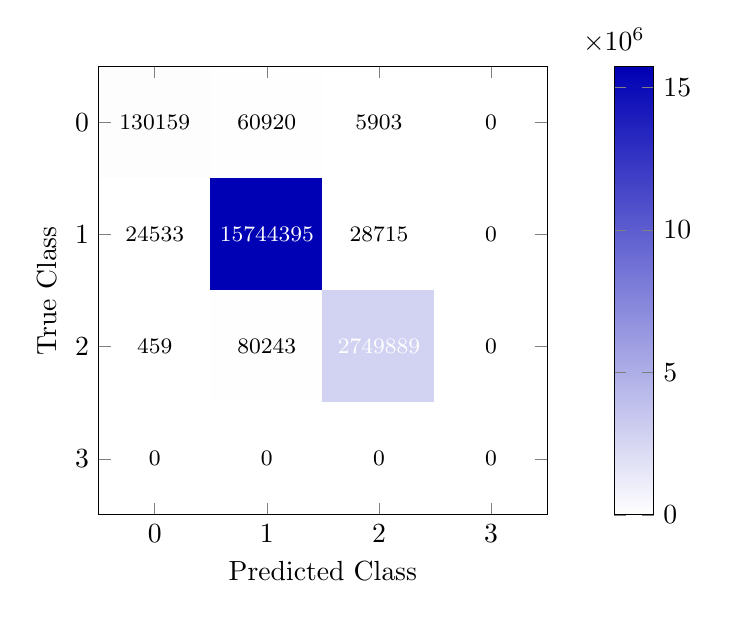
\begin{tikzpicture}
        \begin{axis}[
                width=0.6\textwidth,
                height=0.6\textwidth,
                view={0}{90},
                colormap={whiteblue}{rgb255(0cm)=(255,255,255); rgb255(1cm)=(0,0,180)},
                colorbar right,
                colorbar style={
                        at={(1.15,0.5)},
                        anchor=west,
                        scaled y ticks=base 10:-6,
                        ytick scale label code/.code={$\times 10^{6}$},
                    },
                xlabel={Predicted Class},
                ylabel={True Class},
                xtick={0,1,2,3},
                ytick={0,1,2,3},
                xticklabels={0, 1, 2, 3},
                yticklabels={0, 1, 2, 3},
                y dir=reverse,
                enlargelimits=false,
                point meta min=0,
                point meta max=15744395,
            ]
            \addplot[
                matrix plot,
                mesh/cols=4,
                point meta=explicit,
            ] coordinates {
                    (0,0) [130159]   (1,0) [60920]     (2,0) [5903]      (3,0) [0]
                    (0,1) [24533]    (1,1) [15744395]  (2,1) [28715]     (3,1) [0]
                    (0,2) [459]      (1,2) [80243]     (2,2) [2749889]   (3,2) [0]
                    (0,3) [0]        (1,3) [0]         (2,3) [0]         (3,3) [0]
                };
            % Add numerical labels
            \node at (axis cs:0,0) {\footnotesize 130159};
            \node at (axis cs:1,0) {\footnotesize 60920};
            \node at (axis cs:2,0) {\footnotesize 5903};
            \node at (axis cs:3,0) {\footnotesize 0};
            \node at (axis cs:0,1) {\footnotesize 24533};
            \node[white] at (axis cs:1,1) {\footnotesize 15744395};
            \node at (axis cs:2,1) {\footnotesize 28715};
            \node at (axis cs:3,1) {\footnotesize 0};
            \node at (axis cs:0,2) {\footnotesize 459};
            \node at (axis cs:1,2) {\footnotesize 80243};
            \node[white] at (axis cs:2,2) {\footnotesize 2749889};
            \node at (axis cs:3,2) {\footnotesize 0};
            \node at (axis cs:0,3) {\footnotesize 0};
            \node at (axis cs:1,3) {\footnotesize 0};
            \node at (axis cs:2,3) {\footnotesize 0};
            \node at (axis cs:3,3) {\footnotesize 0};
        \end{axis}
    \end{tikzpicture}
    \caption{Confusion matrix heatmap for baseline segmentation on uncompressed images vs ground truth}
    \label{fig:orig_confusion_matrix}
\end{figure}

An interesting observation from the confusion matrix in Figure \ref{fig:orig_confusion_matrix} is that class 3 does not appear in the test set at all.
This means that the model was never evaluated on this class, which could potentially skew the overall performance. Upon closer inspection, it was found that it doesn't appear once in the whole dataset.
This results in our inability to calculate any meaningful metrics for this class, and thus it was omitted from both Table \ref{tab:orig_seg_metrics} and any future per class metrics tables.
Another observation is that class 0 has a significantly lower occurrence rate compared to classes 1 and 2.
This class imbalance is reflected in the model's performance, with class 0 having notably lower PPV, recall, F1-score, and IoU compared to the other two classes that exist in the dataset.
Overall, the model performs admirably on the uncompressed test dataset, achieving high scores across all metrics.
% Dodac zdjecia
\begin{figure}
    \centering
    \begin{subfigure}{0.3\textwidth}
        \includegraphics[width=\textwidth]{./graf/sample_09_input.png}
        \caption{Original image}
        \label{fig:segmentation_example_original}
    \end{subfigure}
    \hfill
    \begin{subfigure}{0.3\textwidth}
        \includegraphics[width=\textwidth]{./graf/sample_09_gt.png}
        \caption{Ground truth}
        \label{fig:segmentation_example_ground_truth}
    \end{subfigure}
    \hfill
    \begin{subfigure}{0.3\textwidth}
        \includegraphics[width=\textwidth]{./graf/sample_09_pred.png}
        \caption{Predicted segmentation}
        \label{fig:segmentation_example_prediction}
    \end{subfigure}

    \begin{subfigure}{0.3\textwidth}
        \includegraphics[width=\textwidth]{./graf/sample_39_input.png}
        \caption{Original image}
        \label{fig:segmentation_example_original_2}
    \end{subfigure}
    \hfill
    \begin{subfigure}{0.3\textwidth}
        \includegraphics[width=\textwidth]{./graf/sample_39_gt.png}
        \caption{Ground truth}
        \label{fig:segmentation_example_ground_truth_2}
    \end{subfigure}
    \hfill
    \begin{subfigure}{0.3\textwidth}
        \includegraphics[width=\textwidth]{./graf/sample_39_pred.png}
        \caption{Predicted segmentation}
        \label{fig:segmentation_example_prediction_2}
    \end{subfigure}

    \begin{subfigure}{0.3\textwidth}
        \includegraphics[width=\textwidth]{./graf/sample_12_input.png}
        \caption{Original image}
        \label{fig:segmentation_example_original_3}
    \end{subfigure}
    \hfill
    \begin{subfigure}{0.3\textwidth}
        \includegraphics[width=\textwidth]{./graf/sample_12_gt.png}
        \caption{Ground truth}
        \label{fig:segmentation_example_ground_truth_3}
    \end{subfigure}
    \hfill
    \begin{subfigure}{0.3\textwidth}
        \includegraphics[width=\textwidth]{./graf/sample_12_pred.png}
        \caption{Predicted segmentation}
        \label{fig:segmentation_example_prediction_3}
    \end{subfigure}
    \label{fig:segmentation_examples}
    \caption{Examples of semantic segmentation model predictions on uncompressed test images}

\end{figure}
\pagebreak

\section{Compression models evaluation}
\label{sec:eval}
The following subsections describe each model with metrics described in Section \ref{sec:eval_metrics}.
All of the models were evaluated on the test dataset provided in the HySpecNet-11k dataset.
All of the models were assessed using the same set of metrics for consistency and comparability.
Most models were evaluated using the easy split of the dataset, except for the RCGDNAE model, which was evaluated using the hard split.
This choice was made to ensure all of the models were tested under similar conditions, but also to ensure that no data leakage occurred between training and testing phases.
The evaluation metrics used are described in Section \ref{sec:eval_metrics} and include PSNR, SSIM, MSE, SA, bpppc, and compression ratio (CR).
All of the metrics were calculated as mean values over the entire test dataset.
In addition to numerical metrics and histograms of reconstruction errors, several examples of images from the test dataset were selected to visually compare the original and reconstructed images from each model.
Another important aspect of the evaluation was to assess the performance of the semantic segmentation model on the reconstructed images from each compression model.
This was done to measure the impact of compression on downstream tasks such as segmentation.
To this end, the segmentation model described in Chapter \ref{chap:small_segmenter} was used to predict class labels for the reconstructed images from each compression model.
The segmentation model's performance was then evaluated using the metrics described in Section \ref{sec:segmentation_eval}.
This comprehensive evaluation approach allowed for a thorough assessment of each compression model's performance, both in terms of image quality and its impact on downstream tasks.


\subsection{LineRWKV}
The metrics calculated for the LineRWKV model are shown in Table \ref{tab:LineRWKV_metrics}.
The histogram of reconstruction errors for the model is shown in Figure \ref{fig:linerwkv_hist}.
The error map for the best reconstructed image is shown in Figures \ref{fig:linerwkv_best}.\par


\begin{table}[h!]
    \centering
    \caption{LineRWKV evaluation metrics}
    \label{tab:LineRWKV_metrics}
    \begin{tabular}{m{20em}| m{10em}}
        \toprule
        Metric       & Value                  \\
        \midrule
        PSNR (dB)    & 44.87                  \\
        SSIM         & 0.985                  \\
        MSE          & \(3.9 \times 10^{-5}\) \\
        SA (degrees) & 3.987                  \\
        bpppc        & 2.00                   \\
        CR           & 8.00                   \\
        \bottomrule
    \end{tabular}
\end{table}

\begin{figure}
    \centering
    \begin{tikzpicture}
        \begin{axis}[
                width=1\textwidth,
                height=0.8\textwidth,
                xlabel={Reconstruction Error},
                ylabel={Occurrences},
                ybar,
                bar width=1.2pt,
                bar shift=0pt,
                % xtick={-0.02, 0,0.02, 0.04,0.06, 0.08, 0.1, 0.12, 0.13, 0.14, 0.15},
                ymin=0,
                xmin=0,
                grid=major,
            ]
            \addplot [blue, fill=blue]
            table[x index=0, y index=1] {./../results/histograms/LineRWKV.txt};
        \end{axis}
    \end{tikzpicture}
    \caption{Histogram reconstruction error for LineRWKV}
    \label{fig:linerwkv_hist}
\end{figure}


\begin{figure}
    \centering
    \begin{subfigure}{0.45\textwidth}
        \includegraphics[width=\textwidth]{./../results/histograms/RWKV/images/best_original_254.png}
        \caption{Original image}
        \label{fig:linerwkv_best_original}
    \end{subfigure}
    \hfill
    \begin{subfigure}{0.45\textwidth}
        \includegraphics[width=\textwidth]{./../results/histograms/RWKV/images/best_reconstructed_254.png}
        \caption{Reconstructed image}
        \label{fig:linerwkv_best_reconstructed}
    \end{subfigure}
    \par\medskip
    \begin{subfigure}{0.45\textwidth}
        \begin{tikzpicture}
            \node[anchor=south west,inner sep=0] (image) at (0,0) {
                \includegraphics[width=0.85\textwidth]{./../results/histograms/RWKV/images/best_error_map_254_min_-2.196178e-03_max_1.272906e-03.png}
            };
            \begin{axis}[
                at={(image.south east)},
                anchor=south west,
                width=0.12\textwidth,
                height=0.85\textwidth,
                hide axis,
                scale only axis,
                colorbar right,
                colormap={blueblackredzeroed}{
                    color(-2.196178e-03)=(blue);
                    color(0)=(black);
                    color(1.272906e-03)=(red)
                },
                point meta min=-2.196178e-03,
                point meta max=1.272906e-03,
                colorbar style={
                    ylabel={Error},
                    ylabel style={rotate=0}
                }
            ]
            \end{axis}
        \end{tikzpicture}
        \caption{Per pixel error map normalized to between $-2.1962 \times 10^{-3}$ and $1.2729 \times 10^{-3}$}
        \label{fig:linerwkv_best_error_map}
    \end{subfigure}
    \hfill
    \begin{subfigure}{0.5\textwidth}
        \centering
        \begin{tikzpicture}
            \begin{axis}[
                    width=1\textwidth,
                    height=1\textwidth,
                    xlabel={Error},
                    ylabel={Occurrences},
                    ybar,
                bar width=1.2pt,
                bar shift=0pt,
                    ymin=0,
                    grid=major,
                ]
                \addplot [blue, fill=blue]
                table[x index=0, y index=1] {./../results/histograms/RWKV/plots/pixel_error_hist_best_254.txt};
            \end{axis}
        \end{tikzpicture}
        \caption{Per pixel error histogram}
        \label{fig:linerwkv_best_hist}
    \end{subfigure}
    \caption{Best image reconstruction for LineRWKV model}
    \label{fig:linerwkv_best}
\end{figure}

\begin{figure}
    \centering
    \begin{subfigure}{0.45\textwidth}
        \includegraphics[width=\textwidth]{./../results/histograms/RWKV/images/median_original_505.png}
        \caption{Original image}
        \label{fig:linerwkv_mid_original}
    \end{subfigure}
    \hfill
    \begin{subfigure}{0.45\textwidth}
        \includegraphics[width=\textwidth]{./../results/histograms/RWKV/images/median_reconstructed_505.png}
        \caption{Reconstructed image}
        \label{fig:linerwkv_mid_reconstructed}
    \end{subfigure}
    \par\medskip
    \begin{subfigure}{0.45\textwidth}
        \begin{tikzpicture}
            \node[anchor=south west,inner sep=0] (image) at (0,0) {
                \includegraphics[width=0.85\textwidth]{./../results/histograms/RWKV/images/median_error_map_505_min_-4.545168e-03_max_1.904916e-03.png}
            };
            \begin{axis}[
                at={(image.south east)},
                anchor=south west,
                width=0.12\textwidth,
                height=0.85\textwidth,
                hide axis,
                scale only axis,
                colorbar right,
                colormap={blueblackredzeroed}{
                    color(-4.545168e-03)=(blue);
                    color(0)=(black);
                    color(1.904916e-03)=(red)
                },
                point meta min=-4.545168e-03,
                point meta max=1.904916e-03,
                colorbar style={
                    ylabel={Error},
                    ylabel style={rotate=0}
                }
            ]
            \end{axis}
        \end{tikzpicture}
        \caption{Per pixel error map normalized to between $-4.5452 \times 10^{-3}$ and $1.9049 \times 10^{-3}$}
        \label{fig:linerwkv_mid_error_map}
    \end{subfigure}
    \hfill
    \begin{subfigure}{0.5\textwidth}
        \centering
        \begin{tikzpicture}
            \begin{axis}[
                    width=1\textwidth,
                    height=1\textwidth,
                    xlabel={Error},
                    ylabel={Occurrences},
                    ybar,
                bar width=1.2pt,
                bar shift=0pt,
                    ymin=0,
                    grid=major,
                ]
                \addplot [blue, fill=blue]
                table[x index=0, y index=1] {./../results/histograms/RWKV/plots/pixel_error_hist_median_505.txt};
            \end{axis}
        \end{tikzpicture}
        \caption{Per pixel error histogram}
        \label{fig:linerwkv_mid_hist}
    \end{subfigure}
    \caption{Median image reconstruction for LineRWKV model}
    \label{fig:linerwkv_mid}
\end{figure}

\begin{figure}
    \centering
    \begin{subfigure}{0.45\textwidth}
        \includegraphics[width=\textwidth]{./../results/histograms/RWKV/images/worst_original_749.png}
        \caption{Original image}
        \label{fig:linerwkv_worst_original}
    \end{subfigure}
    \hfill
    \begin{subfigure}{0.45\textwidth}
        \includegraphics[width=\textwidth]{./../results/histograms/RWKV/images/worst_reconstructed_749.png}
        \caption{Reconstructed image}
        \label{fig:linerwkv_worst_reconstructed}
    \end{subfigure}
    \par\medskip
    \begin{subfigure}{0.45\textwidth}
        \begin{tikzpicture}
            \node[anchor=south west,inner sep=0] (image) at (0,0) {
                \includegraphics[width=0.85\textwidth]{./../results/histograms/RWKV/images/worst_error_map_749_min_-5.797678e-03_max_3.912130e-03.png}
            };
            \begin{axis}[
                at={(image.south east)},
                anchor=south west,
                width=0.12\textwidth,
                height=0.85\textwidth,
                hide axis,
                scale only axis,
                colorbar right,
                colormap={blueblackredzeroed}{
                    color(-5.797678e-03)=(blue);
                    color(0)=(black);
                    color(3.912130e-03)=(red)
                },
                point meta min=-5.797678e-03,
                point meta max=3.912130e-03,
                colorbar style={
                    ylabel={Error},
                    ylabel style={rotate=0}
                }
            ]
            \end{axis}
        \end{tikzpicture}
        \caption{Per pixel error map normalized to between $-5.7977 \times 10^{-3}$ and $3.9121 \times 10^{-3}$}
        \label{fig:linerwkv_worst_error_map}
    \end{subfigure}
    \hfill
    \begin{subfigure}{0.5\textwidth}
        \centering
        \begin{tikzpicture}
            \begin{axis}[
                    width=1\textwidth,
                    height=1\textwidth,
                    xlabel={Error},
                    ylabel={Occurrences},
                    ybar,
                bar width=1.2pt,
                bar shift=0pt,
                    ymin=0,
                    grid=major,
                ]
                \addplot [blue, fill=blue]
                table[x index=0, y index=1] {./../results/histograms/RWKV/plots/pixel_error_hist_worst_749.txt};
            \end{axis}
        \end{tikzpicture}
        \caption{Per pixel error histogram}
        \label{fig:linerwkv_worst_hist}
    \end{subfigure}
    \caption{Worst image reconstruction for LineRWKV model}
    \label{fig:linerwkv_worst}
\end{figure}




By analyzing the results, it can be assessed that the model is behaving moderately well.
It is able to reconstruct images with high fidelity, as indicated by the high PSNR and SSIM values.
The relatively low PSNR values compared to what would be expected from a lossless or near-lossless compression method stem from the low number of learning epochs used during training.
However, by applying the residuals to the base model predictions, the model is able to achieve near-lossless reconstruction quality.
This, however, comes at a cost to the compression ratio, which is lower than that of other models presented in this thesis. \par
The error histogram in Figure \ref{fig:linerwkv_hist} shows that the majority of reconstruction errors are below \(0.5 \times 10^{-2}\), which indicates that the model is able to reconstruct most images with minimal error.
The error histograms in Figures \ref{fig:linerwkv_best_hist}, \ref{fig:linerwkv_mid_hist}, and \ref{fig:linerwkv_worst_hist} show that the per pixel errors are generally small and in the shape of a normal distribution.
This is generally a good sign, as it shows that the model is good at minimizing large errors, although there exists a slight offset in the error distribution, which can be attributed to the fact that the model is not trained for a sufficient number of epochs to fully converge, which would likely result in a more centered error distribution.
An additional observation from both the histograms and the error maps shown in Figures \ref{fig:linerwkv_best_error_map}, \ref{fig:linerwkv_mid_error_map}, and \ref{fig:linerwkv_worst_error_map} is that there are a few relatively large errors that occur in the reconstructed images, which can be seen in the tails of the error histograms and the red and blue areas in the error maps.
These large errors mostly occur in the beginnings of the images, which is expected, as the model operates on the principle of predicting the next pixel based on the previous ones, which makes the beginning of the images more difficult to reconstruct accurately.\par
The metrics for the segmentation model using the images after compressing and decompressing with the LineRWKV model are shown in tables \ref{tab:seg_metrics_linerwkv} and \ref{tab:seg_metrics_linerwkv_individual}.
These metrics were calculated from the confusion matrix shown in Figure \ref{fig:linerwkv_confusion_matrix}.
The results indicate that the segmentation model performs well on the processed images, albeit with a slight decrease in performance compared to the baseline results on uncompressed images.
This suggests that the LineRWKV model is able to preserve important features in the images that are crucial for downstream tasks such as segmentation.



\begin{table}[h!]
    \centering
    \caption{Average segmentation metrics for LineRWKV reconstructed images}
    \label{tab:seg_metrics_linerwkv}
    \begin{tabular}{m{10em}| m{10em}}
        \toprule
        Metric   & Value  \\
        \midrule
        Accuracy & 0.9645 \\
        F1-score & 0.8394 \\
        IoU      & 0.7490 \\
        AUC      & 0.8674 \\
        \bottomrule
    \end{tabular}
\end{table}

\begin{table}[h!]
    \centering
    \caption{Per class segmentation metrics for LineRWKV reconstructed images}
    \label{tab:seg_metrics_linerwkv_individual}
    \begin{tabular}{m{7em}| m{7em} m{7em} m{7em} m{7em}}
        \toprule
        Metric   & Value for class 0 & Value for class 1 & Value for class 2 \\
        \midrule
        PPV      & 0.6863            & 0.9701            & 0.9478            \\
        Recall   & 0.5974            & 0.9882            & 0.8573            \\
        F1-Score & 0.6388            & 0.9791            & 0.9003            \\
        IoU      & 0.4693            & 0.9590            & 0.8187            \\
        \bottomrule
    \end{tabular}
\end{table}

\begin{figure}[htbp]
    \centering
    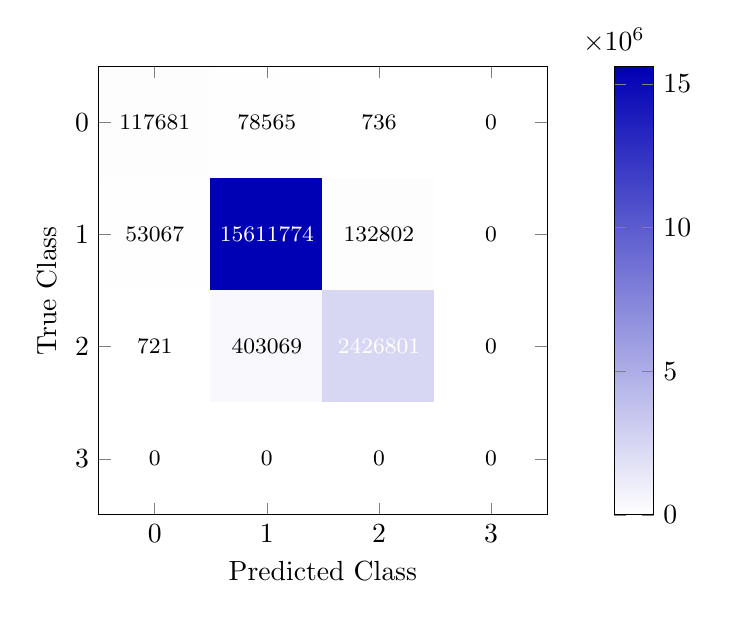
\begin{tikzpicture}
        \begin{axis}[
                width=0.6\textwidth,
                height=0.6\textwidth,
                view={0}{90},
                colormap={whiteblue}{rgb255(0cm)=(255,255,255); rgb255(1cm)=(0,0,180)},
                colorbar right,
                colorbar style={
                        at={(1.15,0.5)},
                        anchor=west,
                        scaled y ticks=base 10:-6,
                        ytick scale label code/.code={$\times 10^{6}$},
                    },
                xlabel={Predicted Class},
                ylabel={True Class},
                xtick={0,1,2,3},
                ytick={0,1,2,3},
                xticklabels={0, 1, 2, 3},
                yticklabels={0, 1, 2, 3},
                y dir=reverse,
                enlargelimits=false,
                point meta min=0,
                point meta max=15611774,
            ]
            \addplot[
                matrix plot,
                mesh/cols=4,
                point meta=explicit,
            ] coordinates {
                    (0,0) [117681]   (1,0) [78565]     (2,0) [736]       (3,0) [0]
                    (0,1) [53067]    (1,1) [15611774]  (2,1) [132802]    (3,1) [0]
                    (0,2) [721]      (1,2) [403069]    (2,2) [2426801]   (3,2) [0]
                    (0,3) [0]        (1,3) [0]         (2,3) [0]         (3,3) [0]
                };
            % Add numerical labels
            \node at (axis cs:0,0) {\footnotesize 117681};
            \node at (axis cs:1,0) {\footnotesize 78565};
            \node at (axis cs:2,0) {\footnotesize 736};
            \node at (axis cs:3,0) {\footnotesize 0};
            \node at (axis cs:0,1) {\footnotesize 53067};
            \node[white] at (axis cs:1,1) {\footnotesize 15611774};
            \node at (axis cs:2,1) {\footnotesize 132802};
            \node at (axis cs:3,1) {\footnotesize 0};
            \node at (axis cs:0,2) {\footnotesize 721};
            \node at (axis cs:1,2) {\footnotesize 403069};
            \node[white] at (axis cs:2,2) {\footnotesize 2426801};
            \node at (axis cs:3,2) {\footnotesize 0};
            \node at (axis cs:0,3) {\footnotesize 0};
            \node at (axis cs:1,3) {\footnotesize 0};
            \node at (axis cs:2,3) {\footnotesize 0};
            \node at (axis cs:3,3) {\footnotesize 0};
        \end{axis}
    \end{tikzpicture}
    \caption{Confusion matrix heatmap for LineRWKV reconstructed images vs ground truth}
    \label{fig:linerwkv_confusion_matrix}
\end{figure}

\pagebreak
\subsection{Residual Convolutional 3D Autoencoder }
The reconstruction results for RCAE3D model are shown in Table \ref{tab:CAE3D_metrics}.
The histogram of reconstruction errors for RCAE3D model is shown in Figure \ref{fig:cae3d_hist}.
The best reconstructed image as well as its error map are shown in Figure \ref{fig:cae3d_best}.\par

\begin{table}[h!]
    \centering
    \caption{RCAE3D evaluation metrics}
    \label{tab:CAE3D_metrics}
    \begin{tabular}{m{20em}| m{10em}}
        \toprule
        Metric       & Value                   \\
        \midrule
        PSNR (dB)    & 38.1504                 \\
        SSIM         & 0.9774                  \\
        MSE          & \(1.89 \times 10^{-4}\) \\
        SA (degrees) & 5.138                   \\
        bpppc        & 1.2673                  \\
        CR           & 12.6253                 \\
        \bottomrule
    \end{tabular}
\end{table}


\begin{figure}[htbp]
    \centering
    \begin{tikzpicture}
        \begin{axis}[
                width=1\textwidth,
                height=0.8\textwidth,
                xlabel={Reconstruction Error},
                ylabel={Occurrences},
                ybar,
                bar width=1.2pt,
                bar shift=0pt,
                xtick={-0.02, 0,0.02, 0.04,0.06, 0.08, 0.1, 0.12, 0.13, 0.14, 0.15},
                ymin=0,
                xmin=0,
                grid=major,
            ]
            \addplot [blue, fill=blue]
            table[x index=0, y index=1] {./graf/cae3D_histogram_data.txt};
        \end{axis}
    \end{tikzpicture}
    \caption{Histogram reconstruction error for RCAE3D}
    \label{fig:cae3d_hist}
\end{figure}


\begin{figure}[htbp]
    \centering
    \begin{subfigure}{0.45\textwidth}
        \includegraphics[width=\textwidth]{./../results/histograms/cae3D/images/best_original_250.png}
        \caption{Original image}
        \label{fig:cae3d_best_original}
    \end{subfigure}
    \hfill
    \begin{subfigure}{0.45\textwidth}
        \includegraphics[width=\textwidth]{./../results/histograms/cae3D/images/best_reconstructed_250.png}
        \caption{Reconstructed image}
        \label{fig:cae3d_best_reconstructed}
    \end{subfigure}
    \par\medskip
    \begin{subfigure}{0.45\textwidth}
        \begin{tikzpicture}
            \node[anchor=south west,inner sep=0] (image) at (0,0) {
                \includegraphics[width=0.85\textwidth]{./../results/histograms/cae3D/images/best_error_map_250_min_-7.727822e-02_max_9.891923e-02.png}
            };
            \begin{axis}[
                at={(image.south east)},
                anchor=south west,
                width=0.12\textwidth,
                height=0.85\textwidth,
                hide axis,
                scale only axis,
                colorbar right,
                colormap={blueblackredzeroed}{
                    color(-7.727822e-02)=(blue);
                    color(0)=(black);
                    color(9.891923e-02)=(red)
                },
                point meta min=-7.727822e-02,
                point meta max=9.891923e-02,
                colorbar style={
                    ylabel={Error},
                    ylabel style={rotate=0}
                }
            ]
            \end{axis}
        \end{tikzpicture}
        \caption{Per pixel error map normalized to between $-7.7278 \times 10^{-2}$ and $9.8919 \times 10^{-2}$}
        \label{fig:cae3d_best_error_map}
    \end{subfigure}
    \hfill
    \begin{subfigure}{0.5\textwidth}
        \centering
        \begin{tikzpicture}
            \begin{axis}[
                    width=1\textwidth,
                    height=1\textwidth,
                    xlabel={Error},
                    ylabel={Occurrences},
                    ybar,
                    bar width=1.2pt,
                    bar shift=0pt,
                    ymin=0,
                    grid=major,
                ]
                \addplot [blue, fill=blue]
                table[x index=0, y index=1] {./../results/histograms/cae3D/plots/pixel_error_hist_best_250.txt};
            \end{axis}
        \end{tikzpicture}
        \caption{Per pixel error histogram}
        \label{fig:cae3d_best_hist}
    \end{subfigure}
    \caption{Best image reconstruction for RCAE3D model}
    \label{fig:cae3d_best}
\end{figure}

\begin{figure}[htbp]
    \centering
    \begin{subfigure}{0.45\textwidth}
        \includegraphics[width=\textwidth]{./../results/histograms/cae3D/images/median_original_132.png}
        \caption{Original image}
        \label{fig:cae3d_mid_original}
    \end{subfigure}
    \hfill
    \begin{subfigure}{0.45\textwidth}
        \includegraphics[width=\textwidth]{./../results/histograms/cae3D/images/median_reconstructed_132.png}
        \caption{Reconstructed image}
        \label{fig:cae3d_mid_reconstructed}
    \end{subfigure}
    \par\medskip
    \begin{subfigure}{0.45\textwidth}
        \begin{tikzpicture}
            \node[anchor=south west,inner sep=0] (image) at (0,0) {
                \includegraphics[width=0.85\textwidth]{./../results/histograms/cae3D/images/median_error_map_132_min_-1.438619e-01_max_2.152214e-01.png}
            };
            \begin{axis}[
                at={(image.south east)},
                anchor=south west,
                width=0.12\textwidth,
                height=0.85\textwidth,
                hide axis,
                scale only axis,
                colorbar right,
                colormap={blueblackredzeroed}{
                    color(-1.438619e-01)=(blue);
                    color(0)=(black);
                    color(2.152214e-01)=(red)
                },
                point meta min=-1.438619e-01,
                point meta max=2.152214e-01,
                colorbar style={
                    ylabel={Error},
                    ylabel style={rotate=0}
                }
            ]
            \end{axis}
        \end{tikzpicture}
        \caption{Per pixel error map normalized to between $-1.4386 \times 10^{-1}$ and $2.1522 \times 10^{-1}$}
        \label{fig:cae3d_mid_error_map}
    \end{subfigure}
    \hfill
    \begin{subfigure}{0.5\textwidth}
        \centering
        \begin{tikzpicture}
            \begin{axis}[
                    width=1\textwidth,
                    height=1\textwidth,
                    xlabel={Error},
                    ylabel={Occurrences},
                    ybar,
                bar width=1.2pt,
                bar shift=0pt,
                    ymin=0,
                    grid=major,
                ]
                \addplot [blue, fill=blue]
                table[x index=0, y index=1] {./../results/histograms/cae3D/plots/pixel_error_hist_median_132.txt};
            \end{axis}
        \end{tikzpicture}
        \caption{Per pixel error histogram}
        \label{fig:cae3d_mid_hist}
    \end{subfigure}
    \caption{Median image reconstruction for RCAE3D model}
    \label{fig:cae3d_mid}
\end{figure}

\begin{figure}[htbp]
    \centering
    \begin{subfigure}{0.45\textwidth}
        \includegraphics[width=\textwidth]{./../results/histograms/cae3D/images/worst_original_323.png}
        \caption{Original image}
        \label{fig:cae3d_worst_original}
    \end{subfigure}
    \hfill
    \begin{subfigure}{0.45\textwidth}
        \includegraphics[width=\textwidth]{./../results/histograms/cae3D/images/worst_reconstructed_323.png}
        \caption{Reconstructed image}
        \label{fig:cae3d_worst_reconstructed}
    \end{subfigure}
    \par\medskip
    \begin{subfigure}{0.45\textwidth}
        \begin{tikzpicture}
            \node[anchor=south west,inner sep=0] (image) at (0,0) {
                \includegraphics[width=0.85\textwidth]{./../results/histograms/cae3D/images/worst_error_map_323_min_-7.757216e-01_max_9.755595e-02.png}
            };
            \begin{axis}[
                at={(image.south east)},
                anchor=south west,
                width=0.12\textwidth,
                height=0.85\textwidth,
                hide axis,
                scale only axis,
                colorbar right,
                colormap={blueblackredzeroed}{
                    color(-7.757216e-01)=(blue);
                    color(0)=(black);
                    color(9.755595e-02)=(red)
                },
                point meta min=-7.757216e-01,
                point meta max=9.755595e-02,
                colorbar style={
                    ylabel={Error},
                    ylabel style={rotate=0}
                }
            ]
            \end{axis}
        \end{tikzpicture}
        \caption{Per pixel error map normalized to between $-7.7572 \times 10^{-1}$ and $9.7556 \times 10^{-2}$}
        \label{fig:cae3d_worst_error_map}
    \end{subfigure}
    \hfill
    \begin{subfigure}{0.5\textwidth}
        \centering
        \begin{tikzpicture}
            \begin{axis}[
                    width=1\textwidth,
                    height=1\textwidth,
                    xlabel={Error},
                    ylabel={Occurrences},
                    ybar,
                bar width=1.2pt,
                bar shift=0pt,
                    ymin=0,
                    grid=major,
                ]
                \addplot [blue, fill=blue]
                table[x index=0, y index=1] {./../results/histograms/cae3D/plots/pixel_error_hist_worst_323.txt};
            \end{axis}
        \end{tikzpicture}
        \caption{Per pixel error histogram}
        \label{fig:cae3d_worst_hist}
    \end{subfigure}
    \caption{Worst image reconstruction for RAE 3D model}
    \label{fig:cae3d_worst}
\end{figure}


\begin{figure}[htbp]
    \centering
    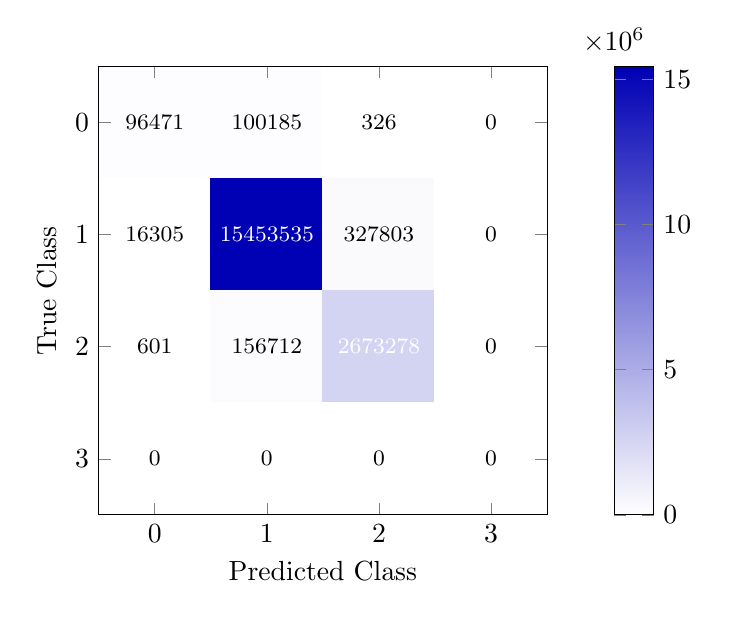
\begin{tikzpicture}
        \begin{axis}[
                width=0.6\textwidth,
                height=0.6\textwidth,
                view={0}{90},
                colormap={whiteblue}{rgb255(0cm)=(255,255,255); rgb255(1cm)=(0,0,180)},
                colorbar right,
                colorbar style={
                        at={(1.15,0.5)},
                        anchor=west,
                        scaled y ticks=base 10:-6,
                        ytick scale label code/.code={$\times 10^{6}$},
                    },
                xlabel={Predicted Class},
                ylabel={True Class},
                xtick={0,1,2,3},
                ytick={0,1,2,3},
                xticklabels={0, 1, 2, 3},
                yticklabels={0, 1, 2, 3},
                y dir=reverse,
                enlargelimits=false,
                point meta min=0,
                point meta max=15453535,
            ]
            \addplot[
                matrix plot,
                mesh/cols=4,
                point meta=explicit,
            ] coordinates {
                    (0,0) [96471]    (1,0) [100185]    (2,0) [326]       (3,0) [0]
                    (0,1) [16305]    (1,1) [15453535]  (2,1) [327803]    (3,1) [0]
                    (0,2) [601]      (1,2) [156712]    (2,2) [2673278]   (3,2) [0]
                    (0,3) [0]        (1,3) [0]         (2,3) [0]         (3,3) [0]
                };
            % Add numerical labels
            \node at (axis cs:0,0) {\footnotesize 96471};
            \node at (axis cs:1,0) {\footnotesize 100185};
            \node at (axis cs:2,0) {\footnotesize 326};
            \node at (axis cs:3,0) {\footnotesize 0};
            \node at (axis cs:0,1) {\footnotesize 16305};
            \node[white] at (axis cs:1,1) {\footnotesize 15453535};
            \node at (axis cs:2,1) {\footnotesize 327803};
            \node at (axis cs:3,1) {\footnotesize 0};
            \node at (axis cs:0,2) {\footnotesize 601};
            \node at (axis cs:1,2) {\footnotesize 156712};
            \node[white] at (axis cs:2,2) {\footnotesize 2673278};
            \node at (axis cs:3,2) {\footnotesize 0};
            \node at (axis cs:0,3) {\footnotesize 0};
            \node at (axis cs:1,3) {\footnotesize 0};
            \node at (axis cs:2,3) {\footnotesize 0};
            \node at (axis cs:3,3) {\footnotesize 0};
        \end{axis}
    \end{tikzpicture}
    \caption{Confusion matrix heatmap for RCAE3D reconstructed images vs ground truth}
    \label{fig:cae3d_confusion_matrix}
\end{figure}


High SSIM and PSNR values indicate that the reconstructed images are very similar to the original ones, both in terms of structure and pixel accuracy.
A low MSE value further confirms that the average squared difference between the original and reconstructed images is minimal.
The SA value indicates that the spectral similarity between the original and reconstructed images is also quite high. \par
At the same time, the histogram \ref{fig:cae3d_hist} shows that most reconstruction errors are concentrated close to zero, with only a few instances of larger errors.
Most of the errors are below \(4 \times 10^{-2}\) with a small additional peak around \(0.11\) which can be attributed to a few outlier images such as the one shown in Figure \ref{fig:cae3d_worst}.
The best reconstructed image shown in Figure \ref{fig:cae3d_best} has a very low error, as can be seen in the error map and the error histogram, which shows that most of the pixel errors are in the range of about \(\pm 1 \times 10^{-2}\).
However, there exists a row of outlier pixels with errors around \(0.1\), which can be clearly seen in the error map in Figure \ref{fig:cae3d_best_error_map}.
These errors most probably occur due to the padding strategy used in the convolutional layers of the model, which can cause some artifacts in the reconstructed images, especially near the borders.
A similar phenomenon can be observed in the other reconstructed images shown in Figures \ref{fig:cae3d_mid} and \ref{fig:cae3d_worst}, where the highest errors occur near the borders of the images, which further supports the hypothesis that these errors are caused by the padding strategy.
\par
In summary, the RCAE3D model demonstrates strong performance in reconstructing images from moderate compression of 1.2673 bpppc and a compression ratio of 12.625, maintaining high fidelity to the original images across multiple evaluation metrics.
The model also has some space for improvement, the validation loss is still decreasing and the model is not overfitted yet. The performance of the segmentation model on the images reconstructed by the RCAE3D model is summarized in tables \ref{tab:seg_metrics_cae3d} and \ref{tab:seg_metrics_cae3d_individual}.
These metrics were calculated from the confusion matrix shown in Figure \ref{fig:cae3d_confusion_matrix}.
The results indicate that the segmentation model handles data processed by the RCAE3D model exquisitely, with only a slight decrease in performance when compared to the baseline.
This suggests that the RCAE3D model is quite effective at preserving spatio-spectral features that are crucial for accurate segmentation, which means that it is suitable for use in practical applications where both compression and segmentation are required.



\begin{table}[h!]
    \centering
    \caption{Average segmentation metrics for RCAE3D reconstructed images}
    \label{tab:seg_metrics_cae3d}
    \begin{tabular}{m{10em}| m{10em}}
        \toprule
        Metric   & Value  \\
        \midrule
        Accuracy & 0.9680 \\
        F1-score & 0.8398 \\
        IoU      & 0.7533 \\
        AUC      & 0.8659 \\
        \bottomrule
    \end{tabular}
\end{table}

\begin{table}[h!]
    \centering
    \caption{Per class segmentation metrics for RCAE3D reconstructed images}
    \label{tab:seg_metrics_cae3d_individual}
    \begin{tabular}{m{7em}| m{7em} m{7em} m{7em} m{7em}}
        \toprule
        Metric   & Value for class 0 & Value for class 1 & Value for class 2 \\
        \midrule
        PPV      & 0.8509            & 0.9836            & 0.8907            \\
        Recall   & 0.4897            & 0.9782            & 0.9444            \\
        F1-Score & 0.6217            & 0.9809            & 0.9168            \\
        IoU      & 0.4510            & 0.9626            & 0.8463            \\
        \bottomrule
    \end{tabular}
\end{table}

\pagebreak
\subsection{Residual Convolutional 2D1D Autoencoder }
The reconstruction metrics for the RCAE2D1D model are shown in Table \ref{tab:CAE2D1D_metrics}.
The histogram of reconstruction errors for the RCAE2D1D model is shown in Figure \ref{fig:cae2d1d_hist}.
The best reconstructed image, as well as its error map are shown in Figure \ref{fig:cae2d1d_best}.\par
Based on the obtained metrics, it can be concluded that the model is performing well, but not as well as the RCAE3D model.
The SSIM and PSNR values are slightly lower than those of the RCAE3D model, indicating that the reconstructed images are less similar to the original ones in terms of structure and pixel accuracy.
The MSE value is higher, which confirms that the average squared difference between the original and reconstructed images is larger.
The SA value is at 6.13 degrees, indicating a moderate level of spectral similarity between the original and reconstructed images.
The compression ratio of this model is 25.09.
\begin{table}[h!]
    \centering
    \caption{RCAE2D1D evaluation metrics}
    \label{tab:CAE2D1D_metrics}
    \begin{tabular}{m{20em}| m{10em}}
        \toprule
        Metric       & Value    \\
        \midrule
        PSNR (dB)    & 34.24    \\
        SSIM         & 0.9619   \\
        MSE          & 0.000487 \\
        SA (degrees) & 6.13     \\
        bpppc        & 0.6337   \\
        CR           & 25.09    \\
        \bottomrule
    \end{tabular}
\end{table}

\begin{figure}[htbp]
    \centering

    \begin{tikzpicture}
        \begin{axis}[
                width=1\textwidth,
                height=0.8\textwidth,
                xlabel={Reconstruction Error},
                ylabel={Occurrences},
                ybar,
                bar width=1.2pt,
                bar shift=0pt,
                xtick={-0.02, 0,0.02, 0.04,0.06, 0.08, 0.1, 0.12, 0.13, 0.14, 0.15},
                ymin=0,
                xmin=0,
                grid=major,
            ]
            \addplot [blue, fill=blue]
            table[x index=0, y index=1] {./graf/cae2D1D_histogram_data.txt};
        \end{axis}
    \end{tikzpicture}
    \caption{Histogram reconstruction error for Residual Convolutional 2D1D Autoencoder }
    \label{fig:cae2d1d_hist}
\end{figure}

\begin{figure}[htbp]
    \centering
    \begin{subfigure}{0.45\textwidth}
        \includegraphics[width=\textwidth]{./../results/histograms/cae2D1D/images/best_original_250.png}
        \caption{Original image}
        \label{fig:cae2d1d_best_original}
    \end{subfigure}
    \hfill
    \begin{subfigure}{0.45\textwidth}
        \includegraphics[width=\textwidth]{./../results/histograms/cae2D1D/images/best_reconstructed_250.png}
        \caption{Reconstructed image}
        \label{fig:cae2d1d_best_reconstructed}
    \end{subfigure}
    \par\medskip
    \begin{subfigure}{0.45\textwidth}
        \begin{tikzpicture}
            \node[anchor=south west,inner sep=0] (image) at (0,0) {
                \includegraphics[width=0.85\textwidth]{./../results/histograms/cae2D1D/images/best_error_map_250_min_-7.725849e-02_max_1.035024e-01.png}
            };
            \begin{axis}[
                at={(image.south east)},
                anchor=south west,
                width=0.12\textwidth,
                height=0.85\textwidth,
                hide axis,
                scale only axis,
                colorbar right,
                colormap={blueblackredzeroed}{
                    color(-7.725849e-02)=(blue);
                    color(0)=(black);
                    color(1.035024e-01)=(red)
                },
                point meta min=-7.725849e-02,
                point meta max=1.035024e-01,
                colorbar style={
                    ylabel={Error},
                    ylabel style={rotate=0}
                }
            ]
            \end{axis}
        \end{tikzpicture}
        \caption{Per pixel error map normalized to between $-7.7258 \times 10^{-2}$ and $1.0350 \times 10^{-1}$}
        \label{fig:cae2d1d_best_error_map}
    \end{subfigure}
    \hfill
    \begin{subfigure}{0.5\textwidth}
        \centering
        \begin{tikzpicture}
            \begin{axis}[
                    width=1\textwidth,
                    height=1\textwidth,
                    xlabel={Error},
                    ylabel={Occurrences},
                    ybar,
                bar width=1.2pt,
                bar shift=0pt,
                    ymin=0,
                    grid=major,
                ]
                \addplot [blue, fill=blue]
                table[x index=0, y index=1] {./../results/histograms/cae2D1D/plots/pixel_error_hist_best_250.txt};
            \end{axis}
        \end{tikzpicture}
        \caption{Per pixel error histogram}
        \label{fig:cae2d1d_best_hist}
    \end{subfigure}
    \caption{Best image reconstruction for RCAE2D1D model}
    \label{fig:cae2d1d_best}
\end{figure}


\begin{figure}[htbp]
    \centering
    \begin{subfigure}{0.45\textwidth}
        \includegraphics[width=\textwidth]{./../results/histograms/cae2D1D/images/median_original_124.png}
        \caption{Original image}
        \label{fig:cae2d1d_mid_original}
    \end{subfigure}
    \hfill
    \begin{subfigure}{0.45\textwidth}
        \includegraphics[width=\textwidth]{./../results/histograms/cae2D1D/images/median_reconstructed_124.png}
        \caption{Reconstructed image}
        \label{fig:cae2d1d_mid_reconstructed}
    \end{subfigure}
    \par\medskip
    \begin{subfigure}{0.45\textwidth}
        \begin{tikzpicture}
            \node[anchor=south west,inner sep=0] (image) at (0,0) {
                \includegraphics[width=0.85\textwidth]{./../results/histograms/cae2D1D/images/median_error_map_124_min_-1.091366e-01_max_8.806012e-02.png}
            };
            \begin{axis}[
                at={(image.south east)},
                anchor=south west,
                width=0.12\textwidth,
                height=0.85\textwidth,
                hide axis,
                scale only axis,
                colorbar right,
                colormap={blueblackredzeroed}{
                    color(-1.091366e-01)=(blue);
                    color(0)=(black);
                    color(8.806012e-02)=(red)
                },
                point meta min=-1.091366e-01,
                point meta max=8.806012e-02,
                colorbar style={
                    ylabel={Error},
                    ylabel style={rotate=0}
                }
            ]
            \end{axis}
        \end{tikzpicture}
        \caption{Per pixel error map normalized to between $-1.0914 \times 10^{-1}$ and $8.8060 \times 10^{-2}$}
        \label{fig:cae2d1d_mid_error_map}
    \end{subfigure}
    \hfill
    \begin{subfigure}{0.5\textwidth}
        \centering
        \begin{tikzpicture}
            \begin{axis}[
                    width=1\textwidth,
                    height=1\textwidth,
                    xlabel={Error},
                    ylabel={Occurrences},
                    ybar,
                    bar width=1.2pt,
                    bar shift=0pt,
                    ymin=0,
                    grid=major,
                ]
                \addplot [blue, fill=blue]
                table[x index=0, y index=1] {./../results/histograms/cae2D1D/plots/pixel_error_hist_median_124.txt};
            \end{axis}
        \end{tikzpicture}
        \caption{Per pixel error histogram}
        \label{fig:cae2d1d_mid_hist}
    \end{subfigure}
    \caption{Mid error image reconstruction for RCAE2D1D model}
    \label{fig:cae2d1d_mid}
\end{figure}


\begin{figure}[htbp]
    \centering
    \begin{subfigure}{0.45\textwidth}
        \includegraphics[width=\textwidth]{./../results/histograms/cae2D1D/images/worst_original_327.png}
        \caption{Original image}
        \label{fig:cae2d1d_worst_original}
    \end{subfigure}
    \hfill
    \begin{subfigure}{0.45\textwidth}
        \includegraphics[width=\textwidth]{./../results/histograms/cae2D1D/images/worst_reconstructed_327.png}
        \caption{Reconstructed image}
        \label{fig:cae2d1d_worst_reconstructed}
    \end{subfigure}
    \par\medskip
    \begin{subfigure}{0.45\textwidth}
        \begin{tikzpicture}
            \node[anchor=south west,inner sep=0] (image) at (0,0) {
                \includegraphics[width=0.85\textwidth]{./../results/histograms/cae2D1D/images/worst_error_map_327_min_-1.911321e-01_max_1.237100e-01.png}
            };
            \begin{axis}[
                at={(image.south east)},
                anchor=south west,
                width=0.12\textwidth,
                height=0.85\textwidth,
                hide axis,
                scale only axis,
                colorbar right,
                colormap={blueblackredzeroed}{
                    color(-1.911321e-01)=(blue);
                    color(0)=(black);
                    color(1.237100e-01)=(red)
                },
                point meta min=-1.911321e-01,
                point meta max=1.237100e-01,
                colorbar style={
                    ylabel={Error},
                    ylabel style={rotate=0}
                }
            ]
            \end{axis}
        \end{tikzpicture}
        \caption{Per pixel error map normalized to between $-1.9113 \times 10^{-1}$ and $1.2371 \times 10^{-1}$}
        \label{fig:cae2d1d_worst_error_map}
    \end{subfigure}
    \hfill
    \begin{subfigure}{0.5\textwidth}
        \centering
        \begin{tikzpicture}
            \begin{axis}[
                    width=1\textwidth,
                    height=1\textwidth,
                    xlabel={Error},
                    ylabel={Occurrences},
                    ybar,
                    bar width=1.2pt,
                    bar shift=0pt,
                    ymin=0,
                    grid=major,
                ]
                \addplot [blue, fill=blue]
                table[x index=0, y index=1] {./../results/histograms/cae2D1D/plots/pixel_error_hist_worst_327.txt};
            \end{axis}
        \end{tikzpicture}
        \caption{Per pixel error histogram}
        \label{fig:cae2d1d_worst_hist}
    \end{subfigure}
    \caption{Worst image reconstruction for RCAE2D1D model}
    \label{fig:cae2d1d_worst}
\end{figure}


\begin{figure}[htbp]
    \centering
    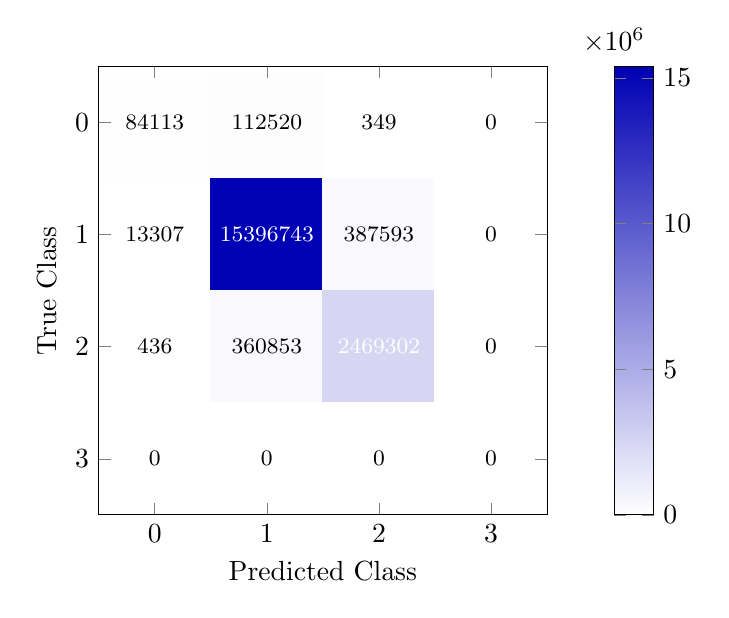
\begin{tikzpicture}
        \begin{axis}[
                width=0.6\textwidth,
                height=0.6\textwidth,
                view={0}{90},
                colormap={whiteblue}{rgb255(0cm)=(255,255,255); rgb255(1cm)=(0,0,180)},
                colorbar right,
                colorbar style={
                        at={(1.15,0.5)},
                        anchor=west,
                        scaled y ticks=base 10:-6,
                        ytick scale label code/.code={$\times 10^{6}$},
                    },
                xlabel={Predicted Class},
                ylabel={True Class},
                xtick={0,1,2,3},
                ytick={0,1,2,3},
                xticklabels={0, 1, 2, 3},
                yticklabels={0, 1, 2, 3},
                y dir=reverse,
                enlargelimits=false,
                point meta min=0,
                point meta max=15396743,
            ]
            \addplot[
                matrix plot,
                mesh/cols=4,
                point meta=explicit,
            ] coordinates {
                    (0,0) [84113]    (1,0) [112520]    (2,0) [349]       (3,0) [0]
                    (0,1) [13307]    (1,1) [15396743]  (2,1) [387593]    (3,1) [0]
                    (0,2) [436]      (1,2) [360853]    (2,2) [2469302]   (3,2) [0]
                    (0,3) [0]        (1,3) [0]         (2,3) [0]         (3,3) [0]
                };
            % Add numerical labels
            \node at (axis cs:0,0) {\footnotesize 84113};
            \node at (axis cs:1,0) {\footnotesize 112520};
            \node at (axis cs:2,0) {\footnotesize 349};
            \node at (axis cs:3,0) {\footnotesize 0};
            \node at (axis cs:0,1) {\footnotesize 13307};
            \node[white] at (axis cs:1,1) {\footnotesize 15396743};
            \node at (axis cs:2,1) {\footnotesize 387593};
            \node at (axis cs:3,1) {\footnotesize 0};
            \node at (axis cs:0,2) {\footnotesize 436};
            \node at (axis cs:1,2) {\footnotesize 360853};
            \node[white] at (axis cs:2,2) {\footnotesize 2469302};
            \node at (axis cs:3,2) {\footnotesize 0};
            \node at (axis cs:0,3) {\footnotesize 0};
            \node at (axis cs:1,3) {\footnotesize 0};
            \node at (axis cs:2,3) {\footnotesize 0};
            \node at (axis cs:3,3) {\footnotesize 0};
        \end{axis}
    \end{tikzpicture}
    \caption{Confusion matrix heatmap for RCAE2D1D reconstructed images vs ground truth}
    \label{fig:cae2d1d_confusion_matrix}
\end{figure}

In summary, the RCAE2D1D model demonstrates decent performance with a slightly higher compression ratio of 25.09 and a bitrate of 0.6337 bpppc, but with a trade-off in reconstruction quality compared to the RCAE3D model.
The histogram \ref{fig:cae2d1d_hist} shows that most errors are concentrated close to zero, with a small additional peak around \(0.13\) which can be attributed to the same outlier images as in the RCAE3D model, such as the one shown in Figure \ref{fig:cae2d1d_worst}.
The histograms and error maps for the best, median, and worst reconstructed images shown in Figures \ref{fig:cae2d1d_best}, \ref{fig:cae2d1d_mid}, and \ref{fig:cae2d1d_worst} respectively, show a similar trend to the RCAE3D model, where the highest errors accumulate near the borders of the images, which can be attributed to the padding strategy used in the convolutional layers of the model.
An additional observation, particularly in the median reconstructed image shown in Figure \ref{fig:cae2d1d_mid}, is that there are some noticeable errors with sudden changes in pixel values, which can be attributed to the fact that the RCAE2D1D model processes the spectral and spatial dimensions separately, which can lead to some loss of information and less accurate reconstructions compared to the RCAE3D model, which processes all dimensions together.
Yet another observation in the error histograms is the skewness of the distribution of errors towards negative values, which can be a result of the model picking up some bias in the training data.
The model is not overfitted; the SSIM and PSNR values are still on the rise, and MSE as well as SA values are still decreasing, indicating that there is still some room for improvement in the model's performance.
\begin{table}[h]
    \centering
    \caption{Average segmentation metrics for RCAE2D1D reconstructed images}
    \label{tab:seg_metrics_cae2d1d}
    \begin{tabular}{m{10em}| m{10em}}
        \toprule
        Metric   & Value  \\
        \midrule
        Accuracy & 0.9535 \\
        F1-score & 0.8037 \\
        IoU      & 0.7042 \\
        AUC      & 0.8610 \\
        \bottomrule
    \end{tabular}
\end{table}

\begin{table}[h]
    \centering
    \caption{Per class segmentation metrics for RCAE2D1D reconstructed images}
    \label{tab:seg_metrics_cae2d1d_individual}
    \begin{tabular}{m{7em}| m{7em} m{7em} m{7em} m{7em}}
        \toprule
        Metric   & Value for class 0 & Value for class 1 & Value for class 2 \\
        \midrule
        PPV      & 0.8596            & 0.9702            & 0.8642            \\
        Recall   & 0.4270            & 0.9746            & 0.8724            \\
        F1-Score & 0.5706            & 0.9724            & 0.8683            \\
        IoU      & 0.3992            & 0.9463            & 0.7672            \\
        \bottomrule
    \end{tabular}
\end{table}

The results of the segmentation model on the images reconstructed by the RCAE2D1D model are summarized in tables \ref{tab:seg_metrics_cae2d1d} and \ref{tab:seg_metrics_cae2d1d_individual}.
These metrics were calculated from the confusion matrix shown in Figure \ref{fig:cae2d1d_confusion_matrix}.
The results indicate that the segmentation model handles data processed by the RCAE2D1D model reasonably well, although there is a more noticeable decrease in performance compared to the baseline than with the RCAE3D model.
This suggests that while the RCAE2D1D model is effective at preserving essential image features for segmentation, it may not retain them as well as other models.
This, however, doesn't disqualify it from practical applications as the results are still acceptable for many use cases where both compression and segmentation are required.


% \pagebreak
\subsection{RCGDNAE}
The RCGDNAE model was evaluated in three different versions, each trained with a different \( \lambda \) parameter.
The models were trained with \( \lambda \) values of 0, 0.001, and 0.01.
These models are called the high, medium, and low bitrate models, respectively.
The reconstruction metrics for RCGDNAE model are shown in Table \ref{tab:RCGDNAE_metrics}.
The histogram of reconstruction errors for RCGDNAE model is shown in Figure \ref{fig:rcgdnae_hist}
The error map for the best reconstructed image is shown in Figure \ref{fig:rcgdnae_low_best_error_map}.\par



\begin{table}[h!]
    \centering
    \caption{RCGDNAE evaluation metrics}
    \label{tab:RCGDNAE_metrics}
    \begin{tabular}{m{10em}| m{7em} m{7em} m{7em}}
        \toprule
        Metric       & Value (High) & Value (Medium) & Value (Low)      \\
        \midrule
        PSNR (dB)    & 38.01        & 36.68          & 37.74            \\
        SSIM         & 0.889        & 0.866          & 0.896            \\
        MSE          & 0.000376     & 0.000469       & 0.000285         \\
        SA (degrees) & 7.47         & 9.27           & 8.89             \\
        bpppc        & 0.015        & 0.0218         & $2.58 * 10^{-5}$ \\
        CR           & 1,036        & 129,799        & 538,667          \\
        \bottomrule
    \end{tabular}
\end{table}

\begin{figure}
    \centering
    \begin{subfigure}[t]{0.45\textwidth}
        \begin{tikzpicture}
            \begin{axis}[
                    width=1\textwidth,
                    height=0.8\textwidth,
                    xlabel={Reconstruction Error},
                    ylabel={Occurrences},
                    ybar,
                bar width=1.2pt,
                bar shift=0pt,
                    ymin=0,
                    xmin=0,
                    grid=major,
                ]
                \addplot [blue, fill=blue]
                table[x index=0, y index=1] {./../results/histograms/high.txt};
            \end{axis}
        \end{tikzpicture}
        \caption{High bitrate}
        \label{fig:rcgdnae_hist_high}
    \end{subfigure}
    \hfill
    \begin{subfigure}[t]{0.45\textwidth}
        \begin{tikzpicture}
            \begin{axis}[
                    width=1\textwidth,
                    height=0.8\textwidth,
                    xlabel={Reconstruction Error},
                    ylabel={Occurrences},
                    ybar,
                bar width=1.2pt,
                bar shift=0pt,
                    ymin=0,
                    xmin=0,
                    grid=major,
                ]
                \addplot [blue, fill=blue]
                table[x index=0, y index=1] {./../results/histograms/mid.txt};
            \end{axis}
        \end{tikzpicture}
        \caption{Medium bitrate}
        \label{fig:rcgdnae_hist_mid}
    \end{subfigure}
    
    \vspace{0.5cm}
    
    \begin{subfigure}{0.45\textwidth}
        \begin{tikzpicture}
            \begin{axis}[
                    width=1\textwidth,
                    height=0.8\textwidth,
                    xlabel={Reconstruction Error},
                    ylabel={Occurrences},
                    ybar,
                bar width=1.2pt,
                bar shift=0pt,
                    ymin=0,
                    xmin=0,
                    grid=major,
                ]
                \addplot [blue, fill=blue]
                table[x index=0, y index=1] {./../results/histograms/low.txt};
            \end{axis}
        \end{tikzpicture}
        \label{fig:rcgdnae_hist_low}
        \caption{Low bitrate}
    \end{subfigure}
    \caption{Mean Aboslute Error histogram for RCGDNAE model per image patch}
    \label{fig:rcgdnae_hist}
\end{figure}

%low RCGDNAE
\begin{figure}
    \centering
    \begin{subfigure}{0.45\textwidth}
        \includegraphics[width=\textwidth]{./../results/histograms/rcgdnae_low/images/best_original_907.png}
        \caption{Original image}
        \label{fig:rcgdnae_low_best_original}
    \end{subfigure}
    \hfill
    \begin{subfigure}{0.45\textwidth}
        \includegraphics[width=\textwidth]{./../results/histograms/rcgdnae_low/images/best_reconstructed_907.png}
        \caption{Reconstructed image}
        \label{fig:rcgdnae_low_best_reconstructed}
    \end{subfigure}
    \par\medskip
    \begin{subfigure}{0.45\textwidth}
        \begin{tikzpicture}
            \node[anchor=south west,inner sep=0] (image) at (0,0) {
                \includegraphics[width=0.85\textwidth]{./../results/histograms/rcgdnae_low/images/best_error_map_907_min_-2.138170e-02_max_1.489278e-02.png}
            };
            \begin{axis}[
                at={(image.south east)},
                anchor=south west,
                width=0.12\textwidth,
                height=0.85\textwidth,
                hide axis,
                scale only axis,
                colorbar right,
                colormap={blueblackredzeroed}{
                    color(-2.138170e-02)=(blue);
                    color(0)=(black);
                    color(1.489278e-02)=(red)
                },
                point meta min=-2.138170e-02,
                point meta max=1.489278e-02,
                colorbar style={
                    ylabel={Error},
                    ylabel style={rotate=0}
                }
            ]
            \end{axis}
        \end{tikzpicture}
        \caption{Per pixel error map normalized to between $-2.1382 \times 10^{-2}$ and $1.4893 \times 10^{-2}$}
        \label{fig:rcgdnae_low_best_error_map}
    \end{subfigure}
    \hfill
    \begin{subfigure}{0.5\textwidth}
        \centering
        \begin{tikzpicture}
            \begin{axis}[
                    width=1\textwidth,
                    height=1\textwidth,
                    xlabel={Error},
                    ylabel={Occurrences},
                    ybar,
                bar width=1.2pt,
                bar shift=0pt,
                    ymin=0,
                    grid=major,
                ]
                \addplot [blue, fill=blue]
                table[x index=0, y index=1] {./../results/histograms/rcgdnae_low/plots/pixel_error_hist_best_907.txt};
            \end{axis}
        \end{tikzpicture}
        \caption{Per pixel error histogram}
        \label{fig:rcgdnae_low_best_hist}
    \end{subfigure}
    \caption{Best image reconstruction for RCGDNAE model (low bitrate)}
    \label{fig:rcgdnae_low_best}
\end{figure}

\begin{figure}
    \centering
    \begin{subfigure}{0.45\textwidth}
        \includegraphics[width=\textwidth]{./../results/histograms/rcgdnae_low/images/median_original_500.png}
        \caption{Original image}
        \label{fig:rcgdnae_low_mid_original}
    \end{subfigure}
    \hfill
    \begin{subfigure}{0.45\textwidth}
        \includegraphics[width=\textwidth]{./../results/histograms/rcgdnae_low/images/median_reconstructed_500.png}
        \caption{Reconstructed image}
        \label{fig:rcgdnae_low_mid_reconstructed}
    \end{subfigure}
    \par\medskip
    \begin{subfigure}{0.45\textwidth}
        \begin{tikzpicture}
            \node[anchor=south west,inner sep=0] (image) at (0,0) {
                \includegraphics[width=0.85\textwidth]{./../results/histograms/rcgdnae_low/images/median_error_map_500_min_-7.874291e-02_max_5.391916e-02.png}
            };
            \begin{axis}[
                at={(image.south east)},
                anchor=south west,
                width=0.12\textwidth,
                height=0.85\textwidth,
                hide axis,
                scale only axis,
                colorbar right,
                colormap={blueblackredzeroed}{
                    color(-7.874291e-02)=(blue);
                    color(0)=(black);
                    color(5.391916e-02)=(red)
                },
                point meta min=-7.874291e-02,
                point meta max=5.391916e-02,
                colorbar style={
                    ylabel={Error},
                    ylabel style={rotate=0}
                }
            ]
            \end{axis}
        \end{tikzpicture}
        \caption{Per pixel error map normalized to between $-7.8742 \times 10^{-2}$ and $5.3919 \times 10^{-2}$}
        \label{fig:rcgdnae_low_mid_error_map}
    \end{subfigure}
    \hfill
    \begin{subfigure}{0.5\textwidth}
        \centering
        \begin{tikzpicture}
            \begin{axis}[
                    width=1\textwidth,
                    height=1\textwidth,
                    xlabel={Error},
                    ylabel={Occurrences},
                    ybar,
                bar width=1.2pt,
                bar shift=0pt,
                    ymin=0,
                    grid=major,
                ]
                \addplot [blue, fill=blue]
                table[x index=0, y index=1] {./../results/histograms/rcgdnae_low/plots/pixel_error_hist_median_500.txt};
            \end{axis}
        \end{tikzpicture}
        \caption{Per pixel error histogram}
        \label{fig:rcgdnae_low_mid_hist}
    \end{subfigure}
    \caption{Median image reconstruction for RCGDNAE model (low bitrate)}
    \label{fig:rcgdnae_low_mid}
\end{figure}

\begin{figure}
    \centering
    \caption{Worst image reconstruction for RCGDNAE model (low bitrate)}
    \label{fig:rcgdnae_low_worst}
    \begin{subfigure}{0.45\textwidth}
        \includegraphics[width=\textwidth]{./../results/histograms/rcgdnae_low/images/worst_original_760.png}
        \caption{Original image}
        \label{fig:rcgdnae_low_worst_original}
    \end{subfigure}
    \hfill
    \begin{subfigure}{0.45\textwidth}
        \includegraphics[width=\textwidth]{./../results/histograms/rcgdnae_low/images/worst_reconstructed_760.png}
        \caption{Reconstructed image}
        \label{fig:rcgdnae_low_worst_reconstructed}
    \end{subfigure}
    \par\medskip
    \begin{subfigure}{0.45\textwidth}
        \begin{tikzpicture}
            \node[anchor=south west,inner sep=0] (image) at (0,0) {
                \includegraphics[width=0.85\textwidth]{./../results/histograms/rcgdnae_low/images/worst_error_map_760_min_-3.361775e-01_max_1.436373e-01.png}
            };
            \begin{axis}[
                at={(image.south east)},
                anchor=south west,
                width=0.12\textwidth,
                height=0.85\textwidth,
                hide axis,
                scale only axis,
                colorbar right,
                colormap={blueblackredzeroed}{
                    color(-3.361775e-01)=(blue);
                    color(0)=(black);
                    color(1.436373e-01)=(red)
                },
                point meta min=-3.361775e-01,
                point meta max=1.436373e-01,
                colorbar style={
                    ylabel={Error},
                    ylabel style={rotate=0}
                }
            ]
            \end{axis}
        \end{tikzpicture}
        \caption{Per pixel error map normalized to between $-3.3618 \times 10^{-1}$ and $1.4364 \times 10^{-1}$}
        \label{fig:rcgdnae_low_worst_error_map}
    \end{subfigure}
    \hfill
    \begin{subfigure}{0.5\textwidth}
        \centering
        \begin{tikzpicture}
            \begin{axis}[
                    width=1\textwidth,
                    height=1\textwidth,
                    xlabel={Error},
                    ylabel={Occurrences},
                    ybar,
                bar width=1.2pt,
                bar shift=0pt,
                    ymin=0,
                    grid=major,
                ]
                \addplot [blue, fill=blue]
                table[x index=0, y index=1] {./../results/histograms/rcgdnae_low/plots/pixel_error_hist_worst_760.txt};
            \end{axis}
        \end{tikzpicture}
        \caption{Per pixel error histogram}
        \label{fig:rcgdnae_low_worst_hist}
    \end{subfigure}
\end{figure}

%mid RCGDNAE
\begin{figure}
    \centering
    \begin{subfigure}{0.45\textwidth}
        \includegraphics[width=\textwidth]{./../results/histograms/rcgdnae_mid/images/best_original_907.png}
        \caption{Original image}
        \label{fig:rcgdnae_mid_best_original}
    \end{subfigure}
    \hfill
    \begin{subfigure}{0.45\textwidth}
        \includegraphics[width=\textwidth]{./../results/histograms/rcgdnae_mid/images/best_reconstructed_907.png}
        \caption{Reconstructed image}
        \label{fig:rcgdnae_mid_best_reconstructed}
    \end{subfigure}
    \par\medskip
    \begin{subfigure}{0.45\textwidth}
        \begin{tikzpicture}
            \node[anchor=south west,inner sep=0] (image) at (0,0) {
                \includegraphics[width=0.85\textwidth]{./../results/histograms/rcgdnae_mid/images/best_error_map_907_min_-2.159815e-02_max_1.726314e-02.png}
            };
            \begin{axis}[
                at={(image.south east)},
                anchor=south west,
                width=0.12\textwidth,
                height=0.85\textwidth,
                hide axis,
                scale only axis,
                colorbar right,
                colormap={blueblackredzeroed}{
                    color(-2.159815e-02)=(blue);
                    color(0)=(black);
                    color(1.726314e-02)=(red)
                },
                point meta min=-2.159815e-02,
                point meta max=1.726314e-02,
                colorbar style={
                    ylabel={Error},
                    ylabel style={rotate=0}
                }
            ]
            \end{axis}
        \end{tikzpicture}
        \caption{Per pixel error map normalized to between $-2.1598 \times 10^{-2}$ and $1.7263 \times 10^{-2}$}
        \label{fig:rcgdnae_mid_best_error_map}
    \end{subfigure}
    \hfill
    \begin{subfigure}{0.5\textwidth}
        \centering
        \begin{tikzpicture}
            \begin{axis}[
                    width=1\textwidth,
                    height=1\textwidth,
                    xlabel={Error},
                    ylabel={Occurrences},
                    ybar,
                bar width=1.2pt,
                bar shift=0pt,
                    ymin=0,
                    grid=major,
                ]
                \addplot [blue, fill=blue]
                table[x index=0, y index=1] {./../results/histograms/rcgdnae_mid/plots/pixel_error_hist_best_907.txt};
            \end{axis}
        \end{tikzpicture}
        \caption{Per pixel error histogram}
        \label{fig:rcgdnae_mid_best_hist}
    \end{subfigure}
    \caption{Best image reconstruction for RCGDNAE model (medium bitrate)}
    \label{fig:rcgdnae_mid_best}
\end{figure}

\begin{figure}
    \centering
    \begin{subfigure}{0.45\textwidth}
        \includegraphics[width=\textwidth]{./../results/histograms/rcgdnae_mid/images/median_original_470.png}
        \caption{Original image}
        \label{fig:rcgdnae_mid_mid_original}
    \end{subfigure}
    \hfill
    \begin{subfigure}{0.45\textwidth}
        \includegraphics[width=\textwidth]{./../results/histograms/rcgdnae_mid/images/median_reconstructed_470.png}
        \caption{Reconstructed image}
        \label{fig:rcgdnae_mid_mid_reconstructed}
    \end{subfigure}
    \par\medskip
    \begin{subfigure}{0.45\textwidth}
        \begin{tikzpicture}
            \node[anchor=south west,inner sep=0] (image) at (0,0) {
                \includegraphics[width=0.85\textwidth]{./../results/histograms/rcgdnae_mid/images/median_error_map_470_min_-1.783785e-01_max_5.689845e-02.png}
            };
            \begin{axis}[
                at={(image.south east)},
                anchor=south west,
                width=0.12\textwidth,
                height=0.85\textwidth,
                hide axis,
                scale only axis,
                colorbar right,
                colormap={blueblackredzeroed}{
                    color(-1.783785e-01)=(blue);
                    color(0)=(black);
                    color(5.689845e-02)=(red)
                },
                point meta min=-1.783785e-01,
                point meta max=5.689845e-02,
                colorbar style={
                    ylabel={Error},
                    ylabel style={rotate=0}
                }
            ]
            \end{axis}
        \end{tikzpicture}
        \caption{Per pixel error map normalized to between $-1.7838 \times 10^{-1}$ and $5.6898 \times 10^{-2}$}
        \label{fig:rcgdnae_mid_mid_error_map}
    \end{subfigure}
    \hfill
    \begin{subfigure}{0.5\textwidth}
        \centering
        \begin{tikzpicture}
            \begin{axis}[
                    width=1\textwidth,
                    height=1\textwidth,
                    xlabel={Error},
                    ylabel={Occurrences},
                    ybar,
                bar width=1.2pt,
                bar shift=0pt,
                    ymin=0,
                    grid=major,
                ]
                \addplot [blue, fill=blue]
                table[x index=0, y index=1] {./../results/histograms/rcgdnae_mid/plots/pixel_error_hist_median_470.txt};
            \end{axis}
        \end{tikzpicture}
        \caption{Per pixel error histogram}
        \label{fig:rcgdnae_mid_mid_hist}
    \end{subfigure}
    \caption{Median image reconstruction for RCGDNAE model (medium bitrate)}
    \label{fig:rcgdnae_mid_mid}
\end{figure}

\begin{figure}
    \centering
    \begin{subfigure}{0.45\textwidth}
        \includegraphics[width=\textwidth]{./../results/histograms/rcgdnae_mid/images/worst_original_760.png}
        \caption{Original image}
        \label{fig:rcgdnae_mid_worst_original}
    \end{subfigure}
    \hfill
    \begin{subfigure}{0.45\textwidth}
        \includegraphics[width=\textwidth]{./../results/histograms/rcgdnae_mid/images/worst_reconstructed_760.png}
        \caption{Reconstructed image}
        \label{fig:rcgdnae_mid_worst_reconstructed}
    \end{subfigure}
    \par\medskip
    \begin{subfigure}{0.45\textwidth}
        \begin{tikzpicture}
            \node[anchor=south west,inner sep=0] (image) at (0,0) {
                \includegraphics[width=0.85\textwidth]{./../results/histograms/rcgdnae_mid/images/worst_error_map_760_min_-3.651287e-01_max_1.368261e-01.png}
            };
            \begin{axis}[
                at={(image.south east)},
                anchor=south west,
                width=0.12\textwidth,
                height=0.85\textwidth,
                hide axis,
                scale only axis,
                colorbar right,
                colormap={blueblackredzeroed}{
                    color(-3.651287e-01)=(blue);
                    color(0)=(black);
                    color(1.368261e-01)=(red)
                },
                point meta min=-3.651287e-01,
                point meta max=1.368261e-01,
                colorbar style={
                    ylabel={Error},
                    ylabel style={rotate=0}
                }
            ]
            \end{axis}
        \end{tikzpicture}
        \caption{Per pixel error map normalized to between $-3.6513 \times 10^{-1}$ and $1.3683 \times 10^{-1}$}
        \label{fig:rcgdnae_mid_worst_error_map}
    \end{subfigure}
    \hfill
    \begin{subfigure}{0.5\textwidth}
        \centering
        \begin{tikzpicture}
            \begin{axis}[
                    width=1\textwidth,
                    height=1\textwidth,
                    xlabel={Error},
                    ylabel={Occurrences},
                    ybar,
                bar width=1.2pt,
                bar shift=0pt,
                    ymin=0,
                    grid=major,
                ]
                \addplot [blue, fill=blue]
                table[x index=0, y index=1] {./../results/histograms/rcgdnae_mid/plots/pixel_error_hist_worst_760.txt};
            \end{axis}
        \end{tikzpicture}
        \caption{Per pixel error histogram}
        \label{fig:rcgdnae_mid_worst_hist}
    \end{subfigure}
    \caption{Worst image reconstruction for RCGDNAE model (medium bitrate)}
    \label{fig:rcgdnae_mid_worst}
\end{figure}

%high RCGDNAE
\begin{figure}
    \centering
    \begin{subfigure}{0.45\textwidth}
        \includegraphics[width=\textwidth]{./../results/histograms/rcgdnae_high/images/best_original_907.png}
        \caption{Original image}
        \label{fig:rcgdnae_high_best_original}
    \end{subfigure}
    \hfill
    \begin{subfigure}{0.45\textwidth}
        \includegraphics[width=\textwidth]{./../results/histograms/rcgdnae_high/images/best_reconstructed_907.png}
        \caption{Reconstructed image}
        \label{fig:rcgdnae_high_best_reconstructed}
    \end{subfigure}
    \par\medskip
    \begin{subfigure}{0.45\textwidth}
        \begin{tikzpicture}
            \node[anchor=south west,inner sep=0] (image) at (0,0) {
                \includegraphics[width=0.85\textwidth]{./../results/histograms/rcgdnae_high/images/best_error_map_907_min_-1.501132e-02_max_1.352057e-02.png}
            };
            \begin{axis}[
                at={(image.south east)},
                anchor=south west,
                width=0.12\textwidth,
                height=0.85\textwidth,
                hide axis,
                scale only axis,
                colorbar right,
                colormap={blueblackredzeroed}{
                    color(-1.501132e-02)=(blue);
                    color(0)=(black);
                    color(1.352057e-02)=(red)
                },
                point meta min=-1.501132e-02,
                point meta max=1.352057e-02,
                colorbar style={
                    ylabel={Error},
                    ylabel style={rotate=0}
                }
            ]
            \end{axis}
        \end{tikzpicture}
        \caption{Per pixel error map normalized to between $-1.5011 \times 10^{-2}$ and $1.3521 \times 10^{-2}$}
        \label{fig:rcgdnae_high_best_error_map}
    \end{subfigure}
    \hfill
    \begin{subfigure}{0.5\textwidth}
        \centering
        \begin{tikzpicture}
            \begin{axis}[
                    width=1\textwidth,
                    height=1\textwidth,
                    xlabel={Error},
                    ylabel={Occurrences},
                    ybar,
                bar width=1.2pt,
                bar shift=0pt,
                    ymin=0,
                    grid=major,
                ]
                \addplot [blue, fill=blue]
                table[x index=0, y index=1] {./../results/histograms/rcgdnae_high/plots/pixel_error_hist_best_907.txt};

            \end{axis}
        \end{tikzpicture}
        \caption{Per pixel error histogram}
        \label{fig:rcgdnae_high_best_hist}
    \end{subfigure}
    \caption{Best image reconstruction for RCGDNAE model (high bitrate)}
    \label{fig:rcgdnae_high_best}
\end{figure}

\begin{figure}
    \centering
    \begin{subfigure}{0.45\textwidth}
        \includegraphics[width=\textwidth]{./../results/histograms/rcgdnae_high/images/median_original_315.png}

        \caption{Original image}
        \label{fig:rcgdnae_high_mid_original}
    \end{subfigure}
    \hfill
    \begin{subfigure}{0.45\textwidth}
        \includegraphics[width=\textwidth]{./../results/histograms/rcgdnae_high/images/median_reconstructed_315.png}
        \caption{Reconstructed image}
        \label{fig:rcgdnae_high_mid_reconstructed}
    \end{subfigure}
    \par\medskip
    \begin{subfigure}{0.45\textwidth}
        \begin{tikzpicture}
            \node[anchor=south west,inner sep=0] (image) at (0,0) {
                \includegraphics[width=0.85\textwidth]{./../results/histograms/rcgdnae_high/images/median_error_map_315_min_-9.686300e-02_max_5.862585e-02.png}
            };
            \begin{axis}[
                at={(image.south east)},
                anchor=south west,
                width=0.12\textwidth,
                height=0.85\textwidth,
                hide axis,
                scale only axis,
                colorbar right,
                colormap={blueblackredzeroed}{
                    color(-9.686300e-02)=(blue);
                    color(0)=(black);
                    color(5.862585e-02)=(red)
                },
                point meta min=-9.686300e-02,
                point meta max=5.862585e-02,
                colorbar style={
                    ylabel={Error},
                    ylabel style={rotate=0}
                }
            ]
            \end{axis}
        \end{tikzpicture}
        \caption{Per pixel error map normalized to between $-9.6863 \times 10^{-2}$ and $5.8626 \times 10^{-2}$}
        \label{fig:rcgdnae_high_mid_error_map}
    \end{subfigure}
    \hfill
    \begin{subfigure}{0.5\textwidth}
        \centering
        \begin{tikzpicture}
            \begin{axis}[
                    width=1\textwidth,
                    height=1\textwidth,
                    xlabel={Error},
                    ylabel={Occurrences},
                    ybar,
                bar width=1.2pt,
                bar shift=0pt,
                    ymin=0,
                    grid=major,
                ]
                \addplot [blue, fill=blue]
                table[x index=0, y index=1] {./../results/histograms/rcgdnae_high/plots/pixel_error_hist_median_315.txt};
            \end{axis}
        \end{tikzpicture}
        \caption{Per pixel error histogram}
        \label{fig:rcgdnae_high_mid_hist}
    \end{subfigure}
    \caption{Median image reconstruction for RCGDNAE model (high bitrate)}
    \label{fig:rcgdnae_high_mid}
\end{figure}

\begin{figure}
    \centering
    \begin{subfigure}{0.45\textwidth}
        \includegraphics[width=\textwidth]{./../results/histograms/rcgdnae_high/images/worst_original_812.png}
        \caption{Original image}
        \label{fig:rcgdnae_high_worst_original}
    \end{subfigure}
    \hfill
    \begin{subfigure}{0.45\textwidth}
        \includegraphics[width=\textwidth]{./../results/histograms/rcgdnae_high/images/worst_reconstructed_812.png}
        \caption{Reconstructed image}
        \label{fig:rcgdnae_high_worst_reconstructed}
    \end{subfigure}
    \par\medskip
    \begin{subfigure}{0.45\textwidth}
        \begin{tikzpicture}
            \node[anchor=south west,inner sep=0] (image) at (0,0) {
                \includegraphics[width=0.85\textwidth]{./../results/histograms/rcgdnae_high/images/worst_error_map_812_min_-3.012457e-01_max_2.306239e-01.png}
            };
            \begin{axis}[
                at={(image.south east)},
                anchor=south west,
                width=0.12\textwidth,
                height=0.85\textwidth,
                hide axis,
                scale only axis,
                colorbar right,
                colormap={blueblackredzeroed}{
                    color(-3.012457e-01)=(blue);
                    color(0)=(black);
                    color(2.306239e-01)=(red)
                },
                point meta min=-3.012457e-01,
                point meta max=2.306239e-01,
                colorbar style={
                    ylabel={Error},
                    ylabel style={rotate=0}
                }
            ]
            \end{axis}
        \end{tikzpicture}
        \caption{Per pixel error map normalized to between $-3.0125 \times 10^{-1}$ and $2.3062 \times 10^{-1}$}
        \label{fig:rcgdnae_high_worst_error_map}
    \end{subfigure}
    \hfill
    \begin{subfigure}{0.5\textwidth}
        \centering
        \begin{tikzpicture}
            \begin{axis}[
                    width=1\textwidth,
                    height=1\textwidth,
                    xlabel={Error},
                    ylabel={Occurrences},
                    ybar,
                bar width=1.2pt,
                bar shift=0pt,
                    ymin=0,
                    grid=major,
                ]
                \addplot [blue, fill=blue]
                table[x index=0, y index=1] {./../results/histograms/rcgdnae_high/plots/pixel_error_hist_worst_812.txt};
            \end{axis}
        \end{tikzpicture}
        \caption{Per pixel error histogram}
        \label{fig:rcgdnae_high_worst_hist}
    \end{subfigure}
    \caption{Worst image reconstruction for RCGDNAE model (high bitrate)}
    \label{fig:rcgdnae_high_worst}
\end{figure}

\begin{figure}[htbp]
    \centering
    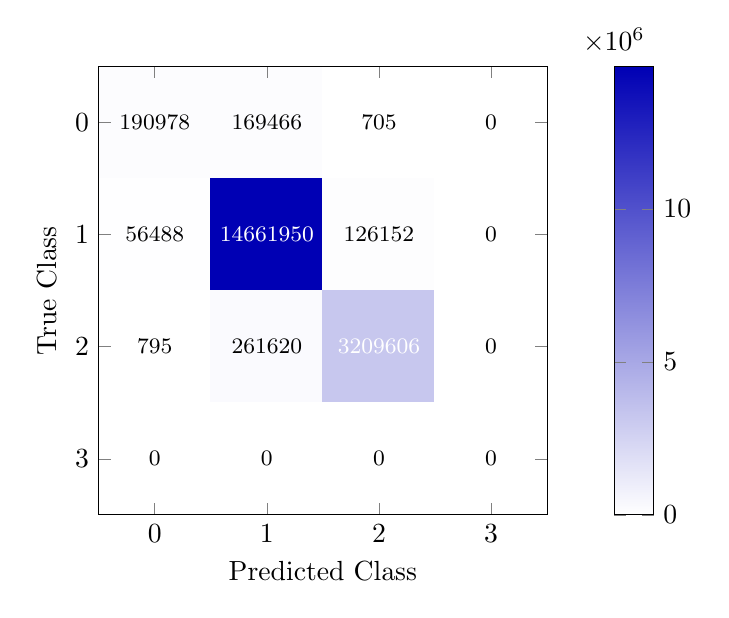
\begin{tikzpicture}
        \begin{axis}[
                width=0.6\textwidth,
                height=0.6\textwidth,
                view={0}{90},
                colormap={whiteblue}{rgb255(0cm)=(255,255,255); rgb255(1cm)=(0,0,180)},
                colorbar right,
                colorbar style={
                        at={(1.15,0.5)},
                        anchor=west,
                        scaled y ticks=base 10:-6,
                        ytick scale label code/.code={$\times 10^{6}$},
                    },
                xlabel={Predicted Class},
                ylabel={True Class},
                xtick={0,1,2,3},
                ytick={0,1,2,3},
                xticklabels={0, 1, 2, 3},
                yticklabels={0, 1, 2, 3},
                y dir=reverse,
                enlargelimits=false,
                point meta min=0,
                point meta max=14661950,
            ]
            \addplot[
                matrix plot,
                mesh/cols=4,
                point meta=explicit,
            ] coordinates {
                    (0,0) [190978]   (1,0) [169466]    (2,0) [705]       (3,0) [0]
                    (0,1) [56488]    (1,1) [14661950]  (2,1) [126152]    (3,1) [0]
                    (0,2) [795]      (1,2) [261620]    (2,2) [3209606]   (3,2) [0]
                    (0,3) [0]        (1,3) [0]         (2,3) [0]         (3,3) [0]
                };
            % Add numerical labels
            \node at (axis cs:0,0) {\footnotesize 190978};
            \node at (axis cs:1,0) {\footnotesize 169466};
            \node at (axis cs:2,0) {\footnotesize 705};
            \node at (axis cs:3,0) {\footnotesize 0};
            \node at (axis cs:0,1) {\footnotesize 56488};
            \node[white] at (axis cs:1,1) {\footnotesize 14661950};
            \node at (axis cs:2,1) {\footnotesize 126152};
            \node at (axis cs:3,1) {\footnotesize 0};
            \node at (axis cs:0,2) {\footnotesize 795};
            \node at (axis cs:1,2) {\footnotesize 261620};
            \node[white] at (axis cs:2,2) {\footnotesize 3209606};
            \node at (axis cs:3,2) {\footnotesize 0};
            \node at (axis cs:0,3) {\footnotesize 0};
            \node at (axis cs:1,3) {\footnotesize 0};
            \node at (axis cs:2,3) {\footnotesize 0};
            \node at (axis cs:3,3) {\footnotesize 0};
        \end{axis}
    \end{tikzpicture}
    \caption{Confusion matrix heatmap for RCGDNAE (low bitrate) reconstructed images vs ground truth}
    \label{fig:rcgdnae_low_confusion_matrix}
\end{figure}

\begin{figure}[htbp]
    \centering
    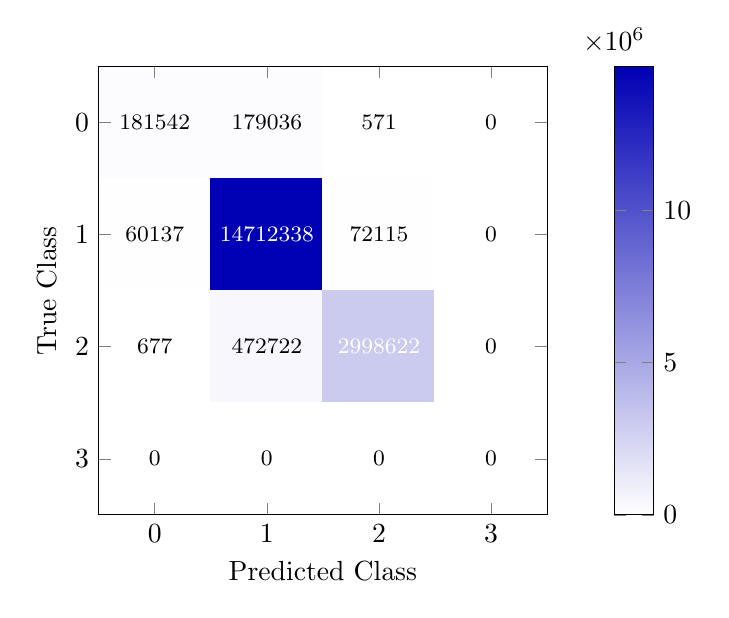
\begin{tikzpicture}
        \begin{axis}[
                width=0.6\textwidth,
                height=0.6\textwidth,
                view={0}{90},
                colormap={whiteblue}{rgb255(0cm)=(255,255,255); rgb255(1cm)=(0,0,180)},
                colorbar right,
                colorbar style={
                        at={(1.15,0.5)},
                        anchor=west,
                        scaled y ticks=base 10:-6,
                        ytick scale label code/.code={$\times 10^{6}$},
                    },
                xlabel={Predicted Class},
                ylabel={True Class},
                xtick={0,1,2,3},
                ytick={0,1,2,3},
                xticklabels={0, 1, 2, 3},
                yticklabels={0, 1, 2, 3},
                y dir=reverse,
                enlargelimits=false,
                point meta min=0,
                point meta max=14712338,
            ]
            \addplot[
                matrix plot,
                mesh/cols=4,
                point meta=explicit,
            ] coordinates {
                    (0,0) [181542]   (1,0) [179036]    (2,0) [571]       (3,0) [0]
                    (0,1) [60137]    (1,1) [14712338]  (2,1) [72115]     (3,1) [0]
                    (0,2) [677]      (1,2) [472722]    (2,2) [2998622]   (3,2) [0]
                    (0,3) [0]        (1,3) [0]         (2,3) [0]         (3,3) [0]
                };
            % Add numerical labels
            \node at (axis cs:0,0) {\footnotesize 181542};
            \node at (axis cs:1,0) {\footnotesize 179036};
            \node at (axis cs:2,0) {\footnotesize 571};
            \node at (axis cs:3,0) {\footnotesize 0};
            \node at (axis cs:0,1) {\footnotesize 60137};
            \node[white] at (axis cs:1,1) {\footnotesize 14712338};
            \node at (axis cs:2,1) {\footnotesize 72115};
            \node at (axis cs:3,1) {\footnotesize 0};
            \node at (axis cs:0,2) {\footnotesize 677};
            \node at (axis cs:1,2) {\footnotesize 472722};
            \node[white] at (axis cs:2,2) {\footnotesize 2998622};
            \node at (axis cs:3,2) {\footnotesize 0};
            \node at (axis cs:0,3) {\footnotesize 0};
            \node at (axis cs:1,3) {\footnotesize 0};
            \node at (axis cs:2,3) {\footnotesize 0};
            \node at (axis cs:3,3) {\footnotesize 0};
        \end{axis}
    \end{tikzpicture}
    \caption{Confusion matrix heatmap for RCGDNAE (mid bitrate) reconstructed images vs ground truth}
    \label{fig:rcgdnae_mid_confusion_matrix}
\end{figure}

\begin{figure}[htbp]
    \centering
    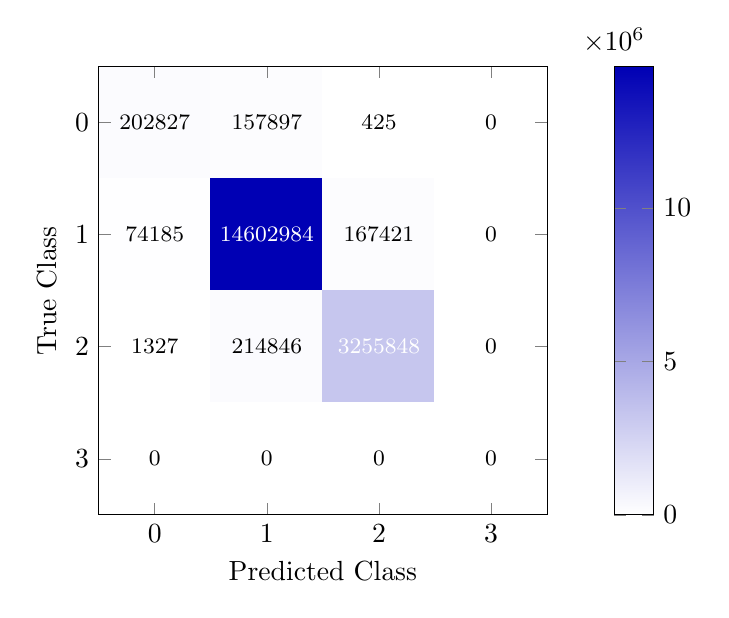
\begin{tikzpicture}
        \begin{axis}[
                width=0.6\textwidth,
                height=0.6\textwidth,
                view={0}{90},
                colormap={whiteblue}{rgb255(0cm)=(255,255,255); rgb255(1cm)=(0,0,180)},
                colorbar right,
                colorbar style={
                        at={(1.15,0.5)},
                        anchor=west,
                        scaled y ticks=base 10:-6,
                        ytick scale label code/.code={$\times 10^{6}$},
                    },
                xlabel={Predicted Class},
                ylabel={True Class},
                xtick={0,1,2,3},
                ytick={0,1,2,3},
                xticklabels={0, 1, 2, 3},
                yticklabels={0, 1, 2, 3},
                y dir=reverse,
                enlargelimits=false,
                point meta min=0,
                point meta max=14602984,
            ]
            \addplot[
                matrix plot,
                mesh/cols=4,
                point meta=explicit,
            ] coordinates {
                    (0,0) [202827]   (1,0) [157897]    (2,0) [425]       (3,0) [0]
                    (0,1) [74185]    (1,1) [14602984]  (2,1) [167421]    (3,1) [0]
                    (0,2) [1327]     (1,2) [214846]    (2,2) [3255848]   (3,2) [0]
                    (0,3) [0]        (1,3) [0]         (2,3) [0]         (3,3) [0]
                };
            % Add numerical labels
            \node at (axis cs:0,0) {\footnotesize 202827};
            \node at (axis cs:1,0) {\footnotesize 157897};
            \node at (axis cs:2,0) {\footnotesize 425};
            \node at (axis cs:3,0) {\footnotesize 0};
            \node at (axis cs:0,1) {\footnotesize 74185};
            \node[white] at (axis cs:1,1) {\footnotesize 14602984};
            \node at (axis cs:2,1) {\footnotesize 167421};
            \node at (axis cs:3,1) {\footnotesize 0};
            \node at (axis cs:0,2) {\footnotesize 1327};
            \node at (axis cs:1,2) {\footnotesize 214846};
            \node[white] at (axis cs:2,2) {\footnotesize 3255848};
            \node at (axis cs:3,2) {\footnotesize 0};
            \node at (axis cs:0,3) {\footnotesize 0};
            \node at (axis cs:1,3) {\footnotesize 0};
            \node at (axis cs:2,3) {\footnotesize 0};
            \node at (axis cs:3,3) {\footnotesize 0};
        \end{axis}
    \end{tikzpicture}
    \caption{Confusion matrix heatmap for RCGDNAE (high bitrate) reconstructed images vs ground truth}
    \label{fig:rcgdnae_high_confusion_matrix}
\end{figure}

The model can achieve extremely high compression ratios, up to 538,667:1 for the low bitrate model.
This, however, comes at a high cost to reconstruction quality.
The extremely low bpppc values initially suggested that there might be an error in the implementation, such as the model being overtrained or data leakage between training and testing datasets.
This is why the model was evaluated using the hard split of the dataset to ensure that no data leakage occurred.
After careful review of the implementation and evaluation process, it was confirmed that the results are accurate and valid.
The high compression ratios achieved by the RCGDNAE model are a result of its architecture, especially the use of the entropy coder, which allows for efficient encoding of the latent representations.
\par
However, the trade-off between compression ratio and reconstruction quality is certainly evident in the results.
All of the reconstructed images show significant loss of detail and introduction of artifacts, especially at lower bitrates.
Upon analysis of the error histograms in Figure \ref{fig:rcgdnae_hist} it is clearly visible that even though the images visually appear to be of very low quality, the majority of errors are actually quite small, with a long tail of larger errors.
This is further reinforced by the distribution of errors in histograms in Figures \ref{fig:rcgdnae_low_mid_hist}, \ref{fig:rcgdnae_low_worst_hist}, \ref{fig:rcgdnae_mid_best_hist}, \ref{fig:rcgdnae_mid_mid_hist}, \ref{fig:rcgdnae_mid_worst_hist}, \ref{fig:rcgdnae_high_best_hist}, \ref{fig:rcgdnae_high_mid_hist}, and \ref{fig:rcgdnae_high_worst_hist}.
Upon visual inspection of the error maps in Figures \ref{fig:rcgdnae_low_mid_error_map}, \ref{fig:rcgdnae_low_worst_error_map}, \ref{fig:rcgdnae_mid_best_error_map}, \ref{fig:rcgdnae_mid_mid_error_map}, \ref{fig:rcgdnae_mid_worst_error_map}, \ref{fig:rcgdnae_high_best_error_map}, \ref{fig:rcgdnae_high_mid_error_map}, and \ref{fig:rcgdnae_high_worst_error_map} it is clear that the errors oscillate around the true pixel values.
This is in contrast to the error maps for the other convolutional autoencoder models, where the errors seem to mostly come from specific regions of the images, such as edges or areas with high intensity gradients.
The reconstructed images themselves show a lack of high frequency details and a general blurring effect, which is consistent with the observed error patterns.\par
The segmentation model was used to quantify the impact of these reconstruction artifacts on downstream tasks.
The confusion matrices for the RCGDNAE reconstructed images against the ground truth segmentations are shown in Figures \ref{fig:rcgdnae_low_confusion_matrix}, \ref{fig:rcgdnae_mid_confusion_matrix}, and \ref{fig:rcgdnae_high_confusion_matrix} for the high, medium, and low bitrate RCGDNAE models, respectively.
The segmentation metrics are reported in Tables \ref{tab:seg_metrics_rcgdnae_high}, \ref{tab:seg_metrics_rcgdnae_mid}, and \ref{tab:seg_metrics_rcgdnae_low}.
The results also include per class metrics in Tables \ref{tab:seg_metrics_rcgdnae_high_individual}, \ref{tab:seg_metrics_rcgdnae_mid_individual}, and \ref{tab:seg_metrics_rcgdnae_low_individual}.
The results show that all compression levels lead to a degradation in segmentation performance compared to the original images.
The error is however much smaller than expected given the visual quality of the reconstructed images, with the low bitrate model achieving an overall accuracy of 0.9671 and an F1-score of 0.8497.
This suggests that while the reconstructed images may look visually poor, they still contain enough information for the segmentation model to perform reasonably well.
This shows that while the usual metrics for image reconstruction quality, such as SSIM and SA, may indicate a significant loss of quality, the reconstructed images can still be useful for downstream tasks such as segmentation.
This is especially important in the context of satellite imagery, where it is conceivable to achieve very high compression ratios while still retaining enough information for certain applications, which can be crucial for efficient storage and transmission of large volumes of satellite data.

%high RCGDNAE
\begin{table}[h!]
    \centering
    \caption{Average segmentation metrics for RCGDNAE (high bitrate) reconstructed images}
    \label{tab:seg_metrics_rcgdnae_high}
    \begin{tabular}{m{10em}| m{10em}}
        \toprule
        Metric   & Value  \\
        \midrule
        Accuracy & 0.9670 \\
        F1-score & 0.8527 \\
        IoU      & 0.7729 \\
        AUC      & 0.8688 \\
        \bottomrule
    \end{tabular}
\end{table}

\begin{table}[h!]
    \centering
    \caption{Per class segmentation metrics for RCGDNAE (high bitrate)  reconstructed images}
    \label{tab:seg_metrics_rcgdnae_high_individual}
    \begin{tabular}{m{7em}| m{7em} m{7em} m{7em} m{7em}}
        \toprule
        Metric   & Value for class 0 & Value for class 1 & Value for class 2 \\
        \midrule
        PPV      & 0.7287            & 0.9751            & 0.9510            \\
        Recall   & 0.5616            & 0.9837            & 0.9377            \\
        F1-Score & 0.6343            & 0.9794            & 0.9443            \\
        IoU      & 0.4645            & 0.9596            & 0.8945            \\
        \bottomrule
    \end{tabular}
\end{table}
%mid RCGDNAE
\begin{table}[h!]
    \centering
    \caption{Average segmentation metrics for RCGDNAE (medium bitrate) reconstructed images}
    \label{tab:seg_metrics_rcgdnae_mid}
    \begin{tabular}{m{10em}| m{10em}}
        \toprule
        Metric   & Value  \\
        \midrule
        Accuracy & 0.9580 \\
        F1-score & 0.8307 \\
        IoU      & 0.7419 \\
        AUC      & 0.8668 \\
        \bottomrule
    \end{tabular}
\end{table}

\begin{table}[h!]
    \centering
    \caption{Per class segmentation metrics for RCGDNAE (medium bitrate) reconstructed images}
    \label{tab:seg_metrics_rcgdnae_mid_individual}
    \begin{tabular}{m{7em}| m{7em} m{7em} m{7em} m{7em}}
        \toprule
        Metric   & Value for class 0 & Value for class 1 & Value for class 2 \\
        \midrule
        PPV      & 0.7491            & 0.9576            & 0.9763            \\
        Recall   & 0.5027            & 0.9911            & 0.8637            \\
        F1-Score & 0.6016            & 0.9740            & 0.9165            \\
        IoU      & 0.4302            & 0.9494            & 0.8459            \\
        \bottomrule
    \end{tabular}
\end{table}
%low RCGDNAE
\begin{table}[h!]
    \centering
    \caption{Average segmentation metrics for RCGDNAE (low bitrate) reconstructed images}
    \label{tab:seg_metrics_rcgdnae_low}
    \begin{tabular}{m{10em}| m{10em}}
        \toprule
        Metric   & Value  \\
        \midrule
        Accuracy & 0.9671 \\
        F1-score & 0.8497 \\
        IoU      & 0.7694 \\
        AUC      & 0.8691 \\
        \bottomrule
    \end{tabular}
\end{table}

\begin{table}[h!]
    \centering
    \caption{Per class segmentation metrics for RCGDNAE (low bitrate) reconstructed images}
    \label{tab:seg_metrics_rcgdnae_low_individual}
    \begin{tabular}{m{7em}| m{7em} m{7em} m{7em} m{7em}}
        \toprule
        Metric   & Value for class 0 & Value for class 1 & Value for class 2 \\
        \midrule
        PPV      & 0.7693            & 0.9714            & 0.9620            \\
        Recall   & 0.5288            & 0.9877            & 0.9244            \\
        F1-Score & 0.6268            & 0.9795            & 0.9428            \\
        IoU      & 0.4564            & 0.9598            & 0.8918            \\
        \bottomrule
    \end{tabular}
\end{table}


\pagebreak
\subsection{Literature reference models}
The models presented in the original papers for each of the reference architectures were used as the baseline for comparison with the models developed in this thesis.
The models presented in the HySpecNet-11k paper\cite{HySpecNet11k} were used, namely the 1D-Convolutional Autoencoder (1D-CAE) (I), Extended 1D-Convolutional Auto-encoder (1D-CAE-Ext) (II), 3D Convolutional Auto-encoder (3D-CAE)(III), and Spectral Signals Compressor Network (SSCNet) (IV).
Additionally, the results presented in the LineRWKV paper\cite{valsesia2024linerwkv}(V) were used as well as for the results presented in the A Scalable Reduced-Complexity Compression of Hyperspectral Remote Sensing Images Using Deep Learning paper\cite{GDN}(VI).
For each of the HySpecNet-11k models, the provided models were run in the validation mode on the easy split of the dataset and the metrics.
For the LineRWKV and Reduced Complexity models, we used the values presented in the original papers.
To keep the comparison simple, we focused on the models with the lowest bpppc values from each paper.
The models were evaluated using the same test dataset and metrics as the models developed in this thesis.
The results of the reference models are presented in Table \ref{tab:reference_models_metrics}
\begin{table}[H]
    \centering
    \caption{Reference models evaluation metrics}
    \label{tab:reference_models_metrics}
    \begin{threeparttable}
        \begin{tabular}{m{8em}| m{3em} m{3em} m{3em} m{3em} m{3em} m{3em}}
            \toprule
            Metric       & I     & II    & III   & IV    & V     & VI     \\
            \midrule
            PSNR (dB)    & 52.52 & 43.22 & 39.06 & 43.91 & 53*   & 61.96  \\
            SSIM         & 0.997 & 0.964 & 0.934 & 0.969 & N/A   & N/A    \\
            SA (degrees) & 1.86  & 5.94  & 5.80  & 3.13  & N/A   & N/A    \\
            bpppc        & 2.06  & 8.08  & 1.00  & 1.00  & 1.4*  & 0.1    \\
            CR           & 7.77  & 1.98  & 16.00 & 16.00 & 11.43 & 160.00 \\
            \bottomrule
        \end{tabular}
        \begin{tablenotes}
            \small
            \item * Value estimated from graph in the original paper.
        \end{tablenotes}
    \end{threeparttable}
\end{table}

It is clearly visible that the models developed in this thesis underperform compared to the reference models from the HySpecNet-11k paper.
This is due to the limited resources available for training and testing the models.
An additional factor that skews the results is the much lower bpppc values achieved by the models developed in this thesis.
The LineRWKV and the Reduced Complexity models could not be directly compared as there had been some difficulties in reproducing the results from the original papers.
